%% 
%% Copyright 2007-2020 Elsevier Ltd
%% 
%% This file is part of the 'Elsarticle Bundle'.
%% ---------------------------------------------
%% 
%% It may be distributed under the conditions of the LaTeX Project Public
%% License, either version 1.2 of this license or (at your option) any
%% later version.  The latest version of this license is in
%%    http://www.latex-project.org/lppl.txt
%% and version 1.2 or later is part of all distributions of LaTeX
%% version 1999/12/01 or later.
%% 
%% The list of all files belonging to the 'Elsarticle Bundle' is
%% given in the file `manifest.txt'.
%% 

%% Template article for Elsevier's document class `elsarticle'
%% with numbered style bibliographic references
%% SP 2008/03/01
%%
%% 
%%
%% $Id: elsarticle-template-num.tex 190 2020-11-23 11:12:32Z rishi $
%%
%%
\documentclass[preprint,12pt]{elsarticle}

%% Use the option review to obtain double line spacing
%% \documentclass[authoryear,preprint,review,12pt]{elsarticle}

%% Use the options 1p,twocolumn; 3p; 3p,twocolumn; 5p; or 5p,twocolumn
%% for a journal layout:
%% \documentclass[final,1p,times]{elsarticle}
%% \documentclass[final,1p,times,twocolumn]{elsarticle}
%% \documentclass[final,3p,times]{elsarticle}
%% \documentclass[final,3p,times,twocolumn]{elsarticle}
%% \documentclass[final,5p,times]{elsarticle}
%% \documentclass[final,5p,times,twocolumn]{elsarticle}

%% For including figures, graphicx.sty has been loaded in
%% elsarticle.cls. If you prefer to use the old commands
%% please give \usepackage{epsfig}

%% The amssymb package provides various useful mathematical symbols
\usepackage{amssymb}
\usepackage{caption}
\usepackage{subcaption}
\usepackage{graphicx} % Required for including pictures
\graphicspath{{Pictures/}} % Specifies the directory where pictures are stored
\usepackage{float}
\usepackage{booktabs}
\usepackage{amsmath}
\usepackage{amsthm}
\usepackage[version=4]{mhchem}
\newtheorem{theorem}{Theorem}

%% The amsthm package provides extended theorem environments
%% \usepackage{amsthm}

%% The lineno packages adds line numbers. Start line numbering with
%% \begin{linenumbers}, end it with \end{linenumbers}. Or switch it on
%% for the whole article with \linenumbers.
%% \usepackage{lineno}

\journal{Applied Energy}

\begin{document}

\begin{frontmatter}

%% Title, authors and addresses

%% use the tnoteref command within \title for footnotes;
%% use the tnotetext command for theassociated footnote;
%% use the fnref command within \author or \address for footnotes;
%% use the fntext command for theassociated footnote;
%% use the corref command within \author for corresponding author footnotes;
%% use the cortext command for theassociated footnote;
%% use the ead command for the email address,
%% and the form \ead[url] for the home page:
%% \title{Title\tnoteref{label1}}
%% \tnotetext[label1]{}
%% \author{Name\corref{cor1}\fnref{label2}}
%% \ead{email address}
%% \ead[url]{home page}
%% \fntext[label2]{}
%% \cortext[cor1]{}
%% \affiliation{organization={},
%%             addressline={},
%%             city={},
%%             postcode={},
%%             state={},
%%             country={}}
%% \fntext[label3]{}

\title{A techno-economic evaluation of decommissioned offshore pipelines as a pressurised gas storage medium for compressed air energy storage}

%% use optional labels to link authors explicitly to addresses:
%% \author[label1,label2]{}
%% \affiliation[label1]{organization={},
%%             addressline={},
%%             city={},
%%             postcode={},
%%             state={},
%%             country={}}
%%
%% \affiliation[label2]{organization={},
%%             addressline={},
%%             city={},
%%             postcode={},
%%             state={},
%%             country={}}

\author[inst1]{Andrew Smallbone}

\affiliation[inst1]{organization={Department of Engineering, University of Durham},%Department and Organization
            addressline={Science Campus}, 
            city={Durham},
            postcode={DH1 3LE}, 
            state={Durham},
            country={UK}}

%\affiliation[inst2]{organization={Department Two},%Department and Organization
%            addressline={Address Two}, 
%            city={City Two},
%            postcode={22222}, 
%            state={State Two},
%            country={Country Two}}

\begin{abstract}
%% Text of abstract
This article presents a techno-economic assessment for the manufacturing, installation, commissioning and operation of large-scale Compressed Air Energy Storage (CAES) systems by recommissioning fossil-fuel era infrastructure as the energy storage medium. It compares the key sensitives of a pipeline-CAES (P-CAES) system in terms of their technical design, technical challenges, implementation, likely costs and its overall value to the energy system in a UK context. A levelised cost evaluation has been employed to show the technology alongside other long-duration energy storage technologies and their potential in terms of scale-up, feasibility and cost. The outcomes show that if deployed in the right locations in the UK, that P-CAES offers a solution which is technically feasible, scale-able etc. with low (potentially the lowest) cost energy storage capacity at the 100MW\textsubscript{e} scale. Furthermore, it is already co-located and embedded into existing energy assets and infrastructure with in-flexible electricity supply and high demand centres. 

\end{abstract}

%%Graphical abstract
\begin{graphicalabstract}

\includegraphics[width=0.8\linewidth]{PCAES-StorageSystem.jpg}
\end{graphicalabstract}

%%Research highlights
\begin{highlights}

\item Compressed air-energy storage can store electrical energy to decarbonise electricity supplies. 
\item The limited number and cost of compressed air storage mediums is a barrier.
\item A techno-economic evaluation has been carried out.
\end{highlights}

\begin{keyword}
%% keywords here, in the form: keyword \sep keyword
Compressed air energy storage \sep Techno-economic evaluation \sep Oil and gas decommissioning
%% PACS codes here, in the form: \PACS code \sep code
\PACS 0000 \sep 1111
%% MSC codes here, in the form: \MSC code \sep code
%% or \MSC[2008] code \sep code (2000 is the default)
\MSC 0000 \sep 1111
\end{keyword}

\end{frontmatter}

%% \linenumbers

%% main text
\section{Introduction}
\label{sec:sample1}
Across all developed and developing nations, achieving a decarbonised electrical energy system will require the roll-out and growth of renewable and inflexible electrical energy supplies \cite{BloombergNEF}. However in order to reach the scale of deployment required, there will be a corresponding negative impact on the resilience, reliability and stability of the electrical and wider energy system. As such, there is a need for solutions for: (1) Addressing future electricity supply and demand imbalances; (2) Changes in conventional geographical transmission flow patterns; and (3) A decrease of electrical system inertia.

The deployment of utility-scale energy storage is hoped to address some of these issues directly by offering additional flexibility to the electricity system. Building upon this, it is anticipated that additional energy storage will complement renewable electricity provision by delivering storage and flexibility across different time spans offering intraday flexibility (less than 12 continuous hours), multiday and multiweek flexibility (12 hours – weeks), seasonal flexibility and flexibility to respond to extreme weather events.

\subsection{Compressed Air Energy Storage}
Compressed Air Energy Storage (CAES), the focus of this article, is a promising grid-scale energy storage method. Energy is stored by converting surplus electrical energy into mechanical potential energy by means of compressing and storing air. At times of high demand, this high-pressure air is fed though an expansion train powering a turbine connected to a generator, feeding power back into the electricity grid. 

Two types of CAES systems are of relevance here: diabatic (D-CAES) and adiabatic (A-CAES), both of which refer to the method by which heat is supplied prior to expansion in the turbine, seen in Figure \ref{fig:caestypes}. The compressed air is stored at ambient temperature to maximise the energy density and reduce thermal stresses on vessel walls \cite{Geissbuhler2018}. To maximise power output, efficiency and to prevent freezing in the turbines, the air must be re-heated before entry to the turbines. Diabatic systems typically re-heat air using a natural gas-powered combustion chamber. Conversely, adiabatic systems store the thermal energy generated by the compression stage using Thermal Energy Storage (TES) systems and use a heat exchanger system to reheat air upon entry to the turbines.

\begin{figure}[H]
    \centering
    \begin{subfigure}[h]{0.45\textwidth}
    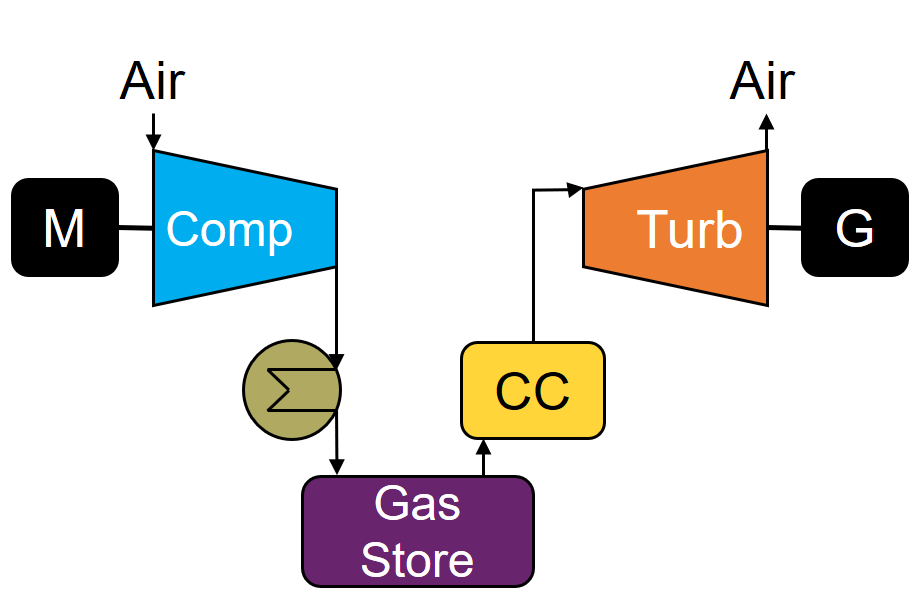
\includegraphics[width=0.9\linewidth]{D-CAES.png}
    \caption{Overall system layout for a Diabatic Compressed Air Energy Storage (D-CAES) plant}
    \label{fig:caestypes-d}
\end{subfigure}
\begin{subfigure}[h]{0.45\textwidth}
    \centering
    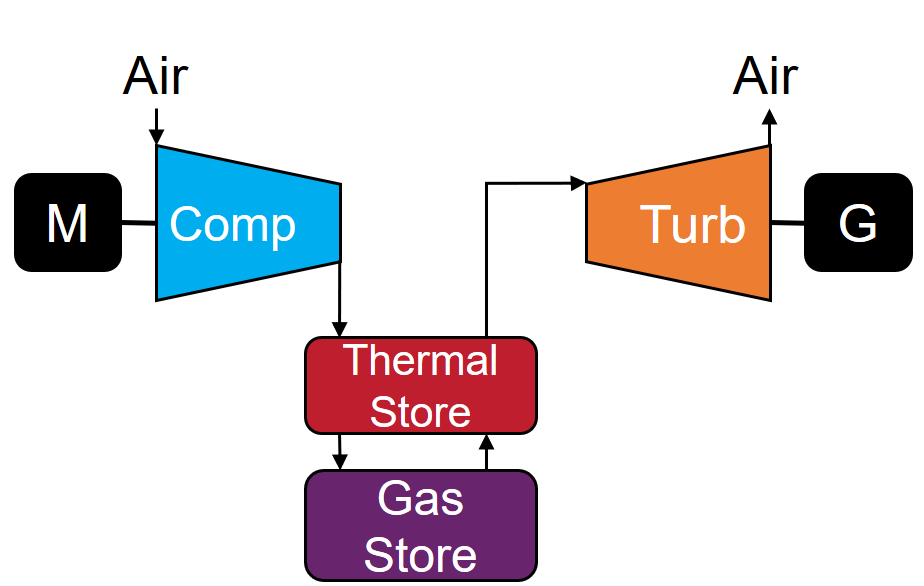
\includegraphics[width=0.9\linewidth]{a-CAES.png}
    \caption{Overall system layout for a Adiabatic Compressed Air Energy Storage (A-CAES) plant}
    \label{fig:caestypes-a}
    \end{subfigure}
    \caption{Block diagram of two common compressed air energy storage (CAES) systems. \textit{M: Motor, Comp: compressor train,  CC: Combustion chamber, Turb: Turbine train, G: Generator.}}
    \label{fig:caestypes}
\end{figure}

Currently, there are two commercialised CAES plants in operation and both adopt the D-CAES configuration. In 1978, a 290 MW plant was built in Huntorf  \cite{Crotogino2001}, Germany, and in 1991 a 110 MW plant was built in McIntosh, Alabama, United States \cite{Luo2014}.  The round-trip efficiency (RTE) of the 310,000m$^3$ Huntorf plant was reported as 42\% \cite{Jafarizadeh2020}. However, the McIntosh plant improved efficiency by implementing a recuperator. Excess heat from the turbine exhaust was used to pre-heat air entering the combustion chamber which improved the RTE to 54\% and reduced fuel consumption by 22-25\% \cite{Budt2016}.

Despite the existence of two commercially successful and operational plants, over recent decades several projects have been proposed \cite{Budt2016} but many have been discontinued due to financial considerations:

\begin{enumerate}
    \item A 220 MW D-CAES plant featuring heat recuperation was planned at the Soyland Power Cooperative Inc., Illinois, US. Construction was ready to commence, and all major equipment was purchased \cite{Linden2007}, however by 1982 a more challenging energy market led to the project being cancelled \cite{Soyland1982}.
    \item	In 2012, a 150 MW D-CAES plant planned by Seneca for the New York ISO was cancelled due to unfavourable energy markets \cite{Rettberg2012}.
    \item 	In 2013, a 2700 MW D-CAES project proposed in Norton, Ohio was cancelled due to increased wholesale energy market prices making the system  economically unfeasible \cite{Budt2016}.
	\item A 300 MW D-CAES plant supplying full load for 10h was planned by PG\&E in California \cite{DOE2014}. The project received \$50m funding from the U.S. Department of Energy and the California Public Utilities Commission but in 2018, after issuing tender, PG\&E found that the best offer could not match other storage technologies. 
	\item	In the UK, Gaelectric proposed a 330MW CAES plant with 6h of rated power. Although the project was awarded €90m of EU funding as a Project of Common Interest (PCI), it was cancelled in 2017 when Gaelectric went into administration \cite{King2021}. 
    
\end{enumerate}

A key part of any CAES system is the compressed air storage (CAS) medium. The most developed storage medium, used in both Huntorf and McIntosh plants, is dissolution-mined salt caverns. These are isochoric (constant volume) CAS systems. The mechanical properties of salt are favourable for high pressure gas storage since the cavern walls can ‘self-heal’ under the pressure exerted by the gas, resulting in very low leakage \cite{Allen1982}. To oppose the force from surrounding rock, a minimum operational pressure must be maintained within the cavern. At Huntorf, this is 20 bar \cite{Crotogino2001}. In Japan, disused mines are the focus of CAS. One successful pilot study was able to achieve storage of pressures up to 80 bar at the Sunagawa cavern, with a volume of 1600m$^2$ \cite{Chen2016}. Underground tunnels have also been the focus of the European Advanced Adiabatic CAES projects. The RICAS2020 \cite{RICAS2020} and ALACAES \cite{Geissbuhler2018} projects have developed CAS in disused mines and underground tunnels. Chen \textit{et al.} \cite{Chen2016} reviewed state-of-the-art CAES systems and highlighted the novel use of steel pipelines as a method of CAS. Notably, a project led by researchers at \textit{Tsinghua University} devised a 100kW steel pipeline CAES system \cite{Chen2016}. It was reported that this achievement confirmed the feasibility of using pipelines in CAES. Valdivia \textit{et al.} \cite{Valdivia2020} completed an assessment into repurposing gas pipelines as the CAS for a grid-scale CAES system in Chile. A techno-economic assessment was made for substations near to existing pipelines and it was found that CAES plants were most profitable connected to power networks with the highest marginal cost variation.

%% The Appendices part is started with the command \appendix;
%% appendix sections are then done as normal sections

\subsection{A decarbonised electrical energy system for net-zero}
\label{sec:decarb}
% Section copied and pasted in---start

%Across all developed and developing nations, achieving a decarbonised electrical energy system will require the roll-out and growth of renewable and inflexible electrical energy supplies. However in order to reach the scale of deployment required, there will be a corresponding negative impact on the resilience, reliability and stability of the electrical and wider energy system. As such, there is a need for solutions for:
%\begin{itemize}
%  \item Addressing future electricity supply and demand imbalances
%  \item Changes in conventional geographical transmission flow patterns; and
%  \item A decrease of electrical system inertia.
%\end{itemize}

%The deployment of utility-scale energy storage is hoped to address some of these issues directly by offering additional flexibility to the electricity system. Building upon this, it is anticipated that additional energy storage will complement renewable electricity provision by delivering storage and flexibility across different time spans:
%\begin{itemize}
%\item Intraday flexibility (<12 continuous hours)
%\item Multiday and multiweek flexibility (12 hours – weeks)
%\item Seasonal flexibility
%\item Flexibility to respond to extreme weather events
%\end{itemize}

%The existing electrical energy system enjoys the benefits of all the above through underpinning its design and operation with an abundance of fossil fuel power generation (principally fuelled by natural gas), or pumped water storage hydropower. Nevertheless, there are an increasing number of deployments of electrochemical batteries at the utility scale. However there are widespread doubts about their potential role for electricity storage over longer durations and their cost effectiveness.

%Hence there is a need to explore, develop and deploy a new generation of powerplants which can deliver flexibility to the wider electrical networks though long-duration energy storage. 

\paragraph{The decarbonisation of our energy system}
Ambitious rates of greenhouse gas (GHG) reduction are required immediately to meet climate change pledges and follow now increasingly more developed decarbonisation pathways. This is a challenge which cuts across our industrialised societies which are complex and interconnected. It requires solutions for all sectors of the economy including for what is expected to be a scaled-up  electricity sector.

In most developed nations, electricity generation is responsible for around a third of their GHG emissions. In 2020, worldwide this represents around 12.3 gigatonnes of carbon dioxide equivalent (Gt CO2eq) \cite{R4}.

However, there are other sectors of developed economies which also require fundamental changes to be decarbonised including transport, residential heat and industry itself, hence the demand for electricity is expected to increase significantly as those sectors transition from fossil fuels and toward other primary energy sources such as renewable electricity. Furthermore an increased world population, and higher living standards in emerging markets and developing economies are likely to drive up electrical demand to as high as three times its current value by 2050 \cite{R4}.

\paragraph{A growing role for renewable power supply}
In recent years, the combined factors of progressive incentives, mass-production, state-driven subsidy alongside a rapid reduction in the price of electricity obtained from wind and solar powered plants has accelerated their roll-out significantly \cite{R3} \cite{hydrogen2030015}. 

In Q2 of 2020, the share of electricity generated from renewable sources was 44.6\% \cite{ENERGYtrends}. This represents an increase of 9\% from 2019, a growth in renewable energy generation that is expected to continue as the UK transitions towards the 2050 Paris agreement. By 2019, energy generated from renewable energy sources (RES) totalled 118.2 TWh and by 2025, the International Energy Agency estimate this will rise to 179.7 TWh \cite{IEAdata}.  Drax Electric Insights estimates that upon reaching 80\% RES generation, a figure required on our path for reaching net zero \cite{cccreport}, 30GW of flexibility from energy storage must be available to the network \cite{SCHMIDT201981}.

As such worldwide, a rapid scale-up of renewable electricity is planned by 2030 with more than 1 terawatts (TW) of installed capacity expected in the electricity sector alone. Nevertheless, this represents a major challenge for the electricity market and wider system which will need to implement more progressive solutions to take advantage of low-cost and abundant renewable power. 

\subsubsection{Long Duration Energy Storage}
The analysis by \textit{McKinsey \& Company} \cite{LDESCouncil} performed in 2021, puts forward a comprehensive case for long-duration energy storage technologies. Their report states that worldwide 5GW and 65GWh of long-duration energy storage is either currently planned or operational. 

They indicate that there is a clear potential for deployment in off-grid systems but overwhelmingly put the main market as energy load shifting, capacity provision and optimisation of transmission and distribution in grid power systems. When coupled to the US electricity market, their analysis shows that the deployment of large volumes of long-duration energy storage would reduce the cost of net-zero power provision by \$35bn by 2040.

By 2040 on a worldwide basis, they expect energy storage capacities to grow by x8-x15 to 1.5-2.5TW and volumes to 85-140TWh. This corresponds to 10\% of all electricity consumed. They also estimate that this would correspond to a cumulative investment of \$1.5-3.0 trillion by 2040. In emissions terms, this would yield a saving or 1.5-2.3 gigatonnes of carbon dioxide equivalent (Gt CO2eq) per year, which is 10-15\% modern power sector emissions. Aggressive targets have been set for 2025, aiming for 30-40GW of capacity and 1.0TWh of storage volume.  

Specifically for the UK, on the 20\textsuperscript{th} July 2021, the Department for Business, Energy and Industrial Strategy (BEIS) announced it is considering evidence on longer-duration energy storage. However whilst we await publication, a 2020 study by \textit{Jacobs} \cite{Jacobs2020} and a 2021 study by \textit{The Association for Renewable Energy \& Clean Technology} \cite{REA2021} have brought further insights. 

The analysis by \textit{Jacobs} \cite{Jacobs2020} utilised UK electrical energy system models to explore net-zero compatible scenarios. They demonstrated the value of additional long-duration storage would have compared to other flexibility options such as more interconnectors. Higher capacities and volumes of long duration storage proved the most cost effective pathways. 

\textit{Jacobs} also recommended that in the UK by 2050, in order to balance 90GW of installed wind power, a long duration energy storage power capacity of 40GW should also be installed with 5,000GWh of storage volume. They suggest that deployment should commence in 10GW stages with the first completed by 2030.

\subsection{Offshore pipelines}
\label{sec:pipelines}

Since the industrial revolution, the UK has sourced most of its energy from fossil fuels \cite{WatersStats}. Vast amounts of infrastructure have been constructed for the extraction, distribution, and storage of these fuels. Looking towards a net-zero future, the application of this infrastructure going forward is uncertain.

\begin{figure}
    \centering
    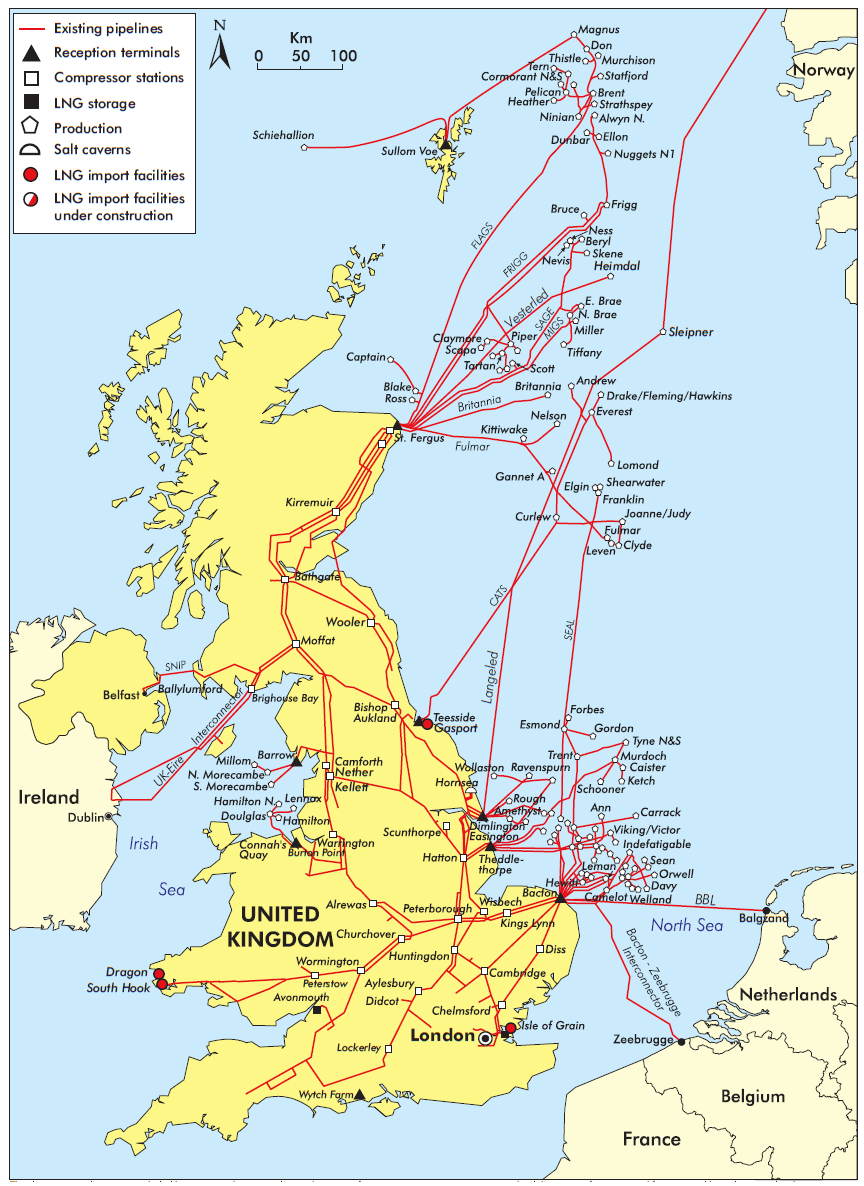
\includegraphics[width = \linewidth]{pipeline.png}
    \caption{Map showing pipelines on the UKCS from \cite{Hall2019}}
    \label{fig:pipelinemap}
\end{figure}

Since the discovery of the Ekofisk Field in 1969 a rapid increase of infrastructure has been built in the North Sea. Oil and gas pipelines totalling 20,000km \cite{OGA2019} connect the UK and mainland Europe to the United Kingdom Continental Shelf (UKCS).  Data obtained from The Oil and Gas Authority (OGA) data explorer \cite{OGAdata} give a greater understanding of the scale of these pipelines. The total volume contained in the North Sea pipelines is 6.21 million standard cubic meters (mscm). Figure \ref{fig:pipelinemap} taken from \cite{pipelinemap} displays the scale of large pipelines operating in the North Sea. Some of the key pipelines of interest are summarised in Table \ref{tab:ukpipes}.  

\begin{table}[H]
    \centering
   \begin{tabular}{lllrr}
\hline
 & Name & UK Connection & Length   {[}km{]} & Volume   {[}m$^3${]} \\ \hline
Gas & Langeled & Easington Section & 543 & 532,946 \\
 & FLAGS & St Fergus & 448 & 294,420 \\
 & SEAL & Bacton & 474 & 277,596 \\
 & CATS & Teesside & 405 & 265,943 \\
 & SAGE & Teesside & 349 & 147,649 \\
Oil & Forties & St Fergus & 324 & 112,002 \\
 & Norpipe & Cruden Bay & 171 & 204,661 \\ \hline
\end{tabular}
    \caption{Key pipelines connected to the UK}
    \label{tab:ukpipes}
\end{table}

Whilst focusing on the Gulf of Mexico, in 2017 Kaiser estimated the costs of the construction of offshore pipelines to be around \$2m/km \cite{KAISER2017147}. 

The vast majority of offshore pipelines are made from high-yield steel which can carry liquids or gases at high pressure and can be rated up to 350-500MPa. There are a variety of diameters which have been deployed from 3 to 54 inches (0.076–1.37m) with thicknesses from 0.25 to 1.5 in (6–38 mm). Typically offshore pipelines are constructed from rigid 12m long segments of pipe which are welded together and then laid on the seabed using a pipeline lay vessel.

The full Langeled Pipeline located in the North Sea connects Nyhamna, Norway to Easington, UK via a 1167km 44 inch (1.12m) diameter (25mm thickness) gas pipeline costing \$3.8m/km \cite{KaieteurNews2021}. It is constructed from 100,000 sections coated in asphalt and concrete and was laid at up to 8km/day. The UK's offshore pipelines vary in diameter from 18 inches (0.457m) to 44 inches (1.12m) and are mainly made from low alloy carbon steel with higher ally metals now increasingly been deployed \cite {HSE}. The operating pressure range for a long offshore gas transmission pipeline is very wide but typically between an upstream pressure of 150–250 bar, and a downstream pressure of 60 to 80 bar over a distance of several hundred kilometers \cite{Campbell}. 

\subsubsection{Offshore pipeline lifetime}

The \textit{UK's Health and Safety Executive} \cite {HSE} have a set of guidelines around the lifetime of offshore pipelines. Many North Sea pipelines have been in place for longer than their original 20-30 year lifetimes and are inspected before extending their working lifetime. Many will may have some unique characteristics in terms of material, wall thickness, anti-corrosion coating, concrete coating and degree of burial and these may well factor in their rate of corrosion as well as damage from external sources. 

Cathodic protection is the most effective mode for protection which quickly reaches an equilibrium which can be maintained for many years, nevertheless anti-corrosion coatings do slowly deteriorate with time. It is considered that rates of corrosion can be managed using these mechanisms and inspection. However once the Cathodic protection no longer functions, the rate of corrosion increases, a 12mm thickness well maintained steel pipeline on the surface would be expected to last 60 years and a buried one for 400 years.

\subsection{Offshore pipeline decommissioning and abandonment}
The process of pipeline decommissioning (and abandonment) is carried out if: 
\begin{enumerate}
  \item It is no longer required and has expired its useful lifetime or is no long economically viable.
  \item Reserves of oil/gas are exhausted.
\end{enumerate}

The formal decommissioning of a pipelines makes sure that all the components of a pipe network are safely dismantled (or neutralised) to prevent establishing an unwanted long lasting environmental hazard. Normally this requires purging the pipeline with nitrogen, pigging (cleaning inspecting and purging), filling and plugging.

Another relevant term is pipeline abandonment which is a form of decommissioning, this aims to keep much of the infrastructure in place whilst removing combustible fluids, disconnecting and sealing it up.

\textit{Oil and Gas UK (OGUK)} prepare annual reports on the state of the UK's oil and gas infrastructure. Whilst the UK's net gas production exceeded 65 bn m\textsuperscript{3} in 2008 by 2030 this could be as low as 20 bn m\textsuperscript{3} \cite{Hall2019}. As such, rapid decommissioning is underway. One of their most recent, ‘Decommissioning insights 2020’ \cite{OGUKdecom} details the decommissioning of some 260km of pipeline, a small part of a decommissioning endeavour that cost £1.08bn. A more recent 2021 report \cite{OGA2021}, sets out the expected expenditure on decommissioning in the UK out to 2066. As shown in Figure \ref{fig:decomiss}, expenditure is expected to rise over the next decade to around £1.5bn/year before rising to over £2.0bn/year until 2040. 

\begin{figure}
    \centering
    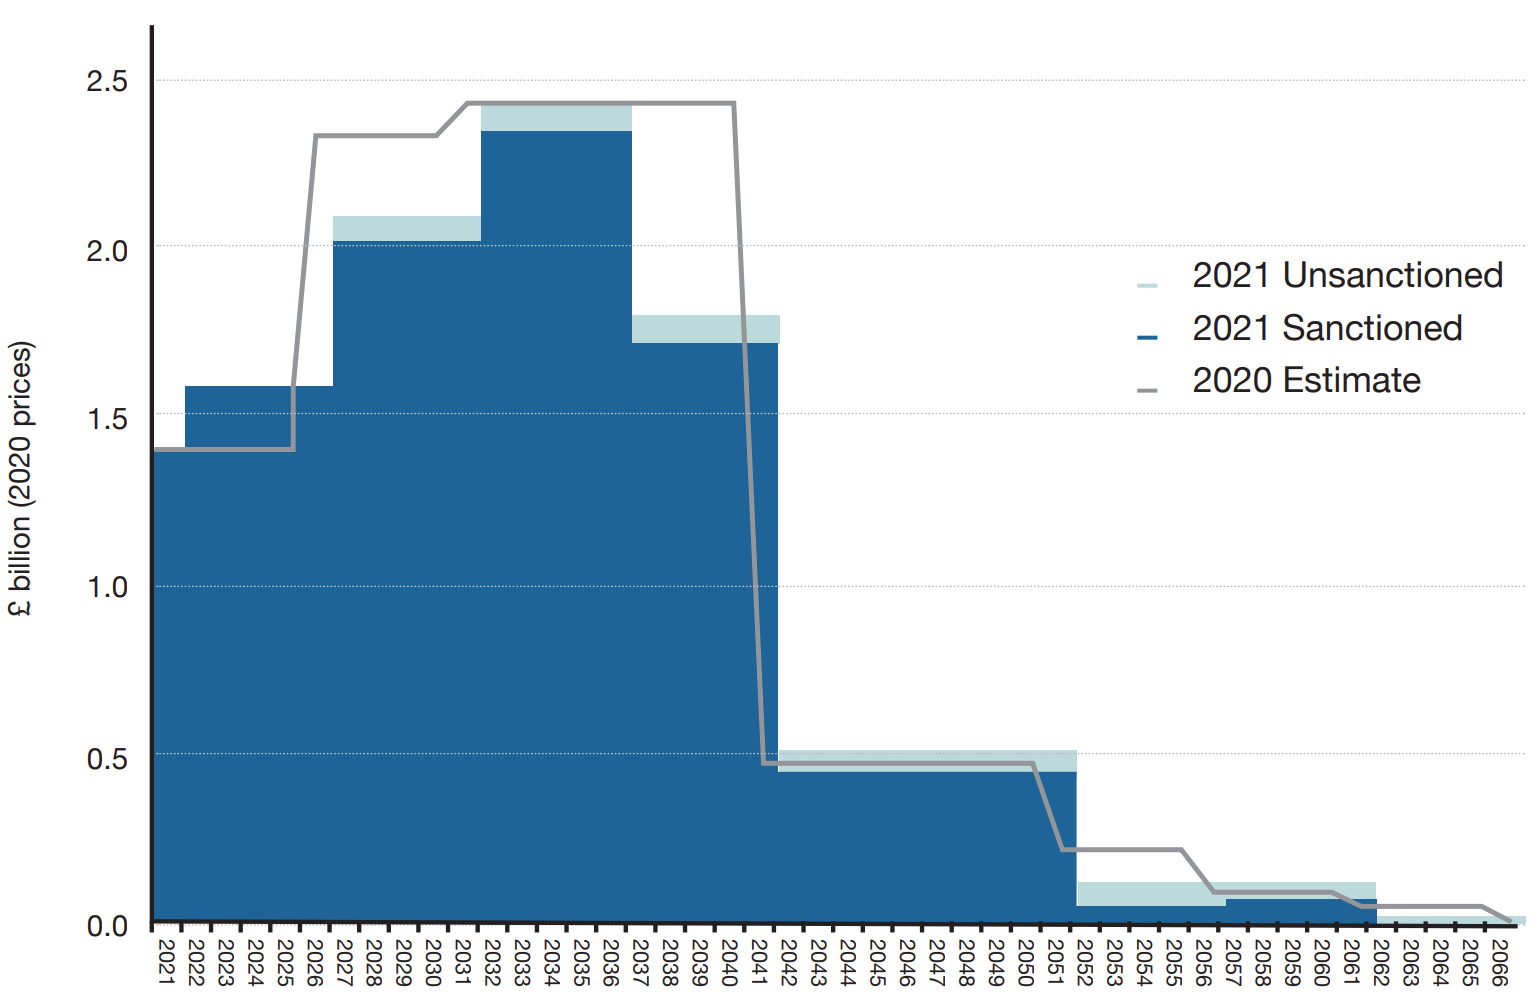
\includegraphics[width = 12cm ]{decomissioning.png}
    \caption{Projected Annual UK Continental Shelf Decommissioning Costs, July 2021 \cite{OGA2021}}
    \label{fig:decomiss}
\end{figure}

One alternative option is to avoid decommissioning and to repurpose this infrastructure for utilisation for other applications other than transporting fossil fuels. The OGUK report \cite{OGA2021} notes this as an area of "increasing focus" with emerging opportunities for carbon capture and storage, hydrogen and renewables. None of these have been considered or are included in the decommissioning cost estimates put forward.

\subsection{Opportunities beyond the UK's coastline}

In December 2020, as presented in Table \ref{fig:NumPipes} there were 22 retired pipelines and over 2300 operational pipelines across the world. In practice, to meet internationally agreed targets for greenhouse gas emissions or by virtue that extraction is no longer viable, many of these will ultimately need to be decommissioned or repurposed for other applications. 

As in the North Sea, the proposed solution for energy storage remains a potential option. Offshore pipelines can last significantly longer than their original design lifetime especially when well maintained. Rebalancing intermittent renewable or nuclear power is a challenge that needs to be addressed in almost all regions and as such the proposed solution could be in principal be exported internationally.

\begin{table}[]
    \centering
\begin{tabular}{||l c c ||} 
 \hline
\textbf{Current Status} & \textbf{Oil} & \textbf{Gas} \\ 
  \hline
 Proposed & 69 & 342\\ 
 Under construction &33 & 121\\ 
 Shelved & 20 & 52\\ 
 Cancelled & 58 & 132\\ 
 \hline
 Operating & 649 & 1732\\ 
 \hline
 Mothballed/Retired & 11 & 11\\ 
 \hline
\end{tabular}
\caption{Worldwide pipeline numbers and status as of December 2020 (Source: Statista)}
\label{fig:NumPipes}

\end{table}

Whilst it is clear that many of the 2300 operational pipelines will face decommissioning in the next 20-30 years, the precise timing of these events is regionally and nationally dependent and associated with political factors, the aggressiveness of decarbonisation planned, current state of the infrastructure and availability of fossil reserves. 

\section{Technical approach}

The proposed project aims to explore recommissioning some of the UKCS pipeline infrastructure as the CAS vessel for a CAES system. A schematic of such a system is presented in Figure \ref{fig:P_CAES}. 

\begin{figure}
    \centering
    
\includegraphics[width=0.8\linewidth]{PCAES-StorageSystem.jpg}
    \caption{Infographic detailing a compressed air energy storage (CAES) system coupled to an offshore pipeline}
    \label{fig:P_CAES}
\end{figure}

An air compressor and expansion turbine plant must be constructed on the land-side of the pipeline. When the local electricity market has excess supply, the pipeline is filled with compressed air. The length of the pipe will be used as the main gas storage medium with the distant end sealed off at an appropriate length. When there is a shortage of electricity, the compressed gas is used to power the expansion turbine.

\subsection{Offshore pipelines}
A schematic of an offshore subsea pipeline is presented in Figure \ref{fig:PipeForces}. 

The figure shows the external forces which act upon the pipeline segment, these include water-induced hydrodynamic forces including waves and current, the weight of the pipeline itself, and the soil resistance. Pipelines typically lay directly upon the seabed although they are often cemented into place or installed in an artificial trench (and back filled). Depending upon factors influencing the original lay of the pipe \cite{YU2013598}, over time  pipe-soil interaction will influence pipeline lateral stability. Also, the loading and unloading of pressure within the pipe itself can over long distances cause significant lateral movements of the pipeline. However, the monitoring of pipeline integrity and any risks to their failure is commonplace in the offshore sector.

\begin{figure}[b]
    \centering
    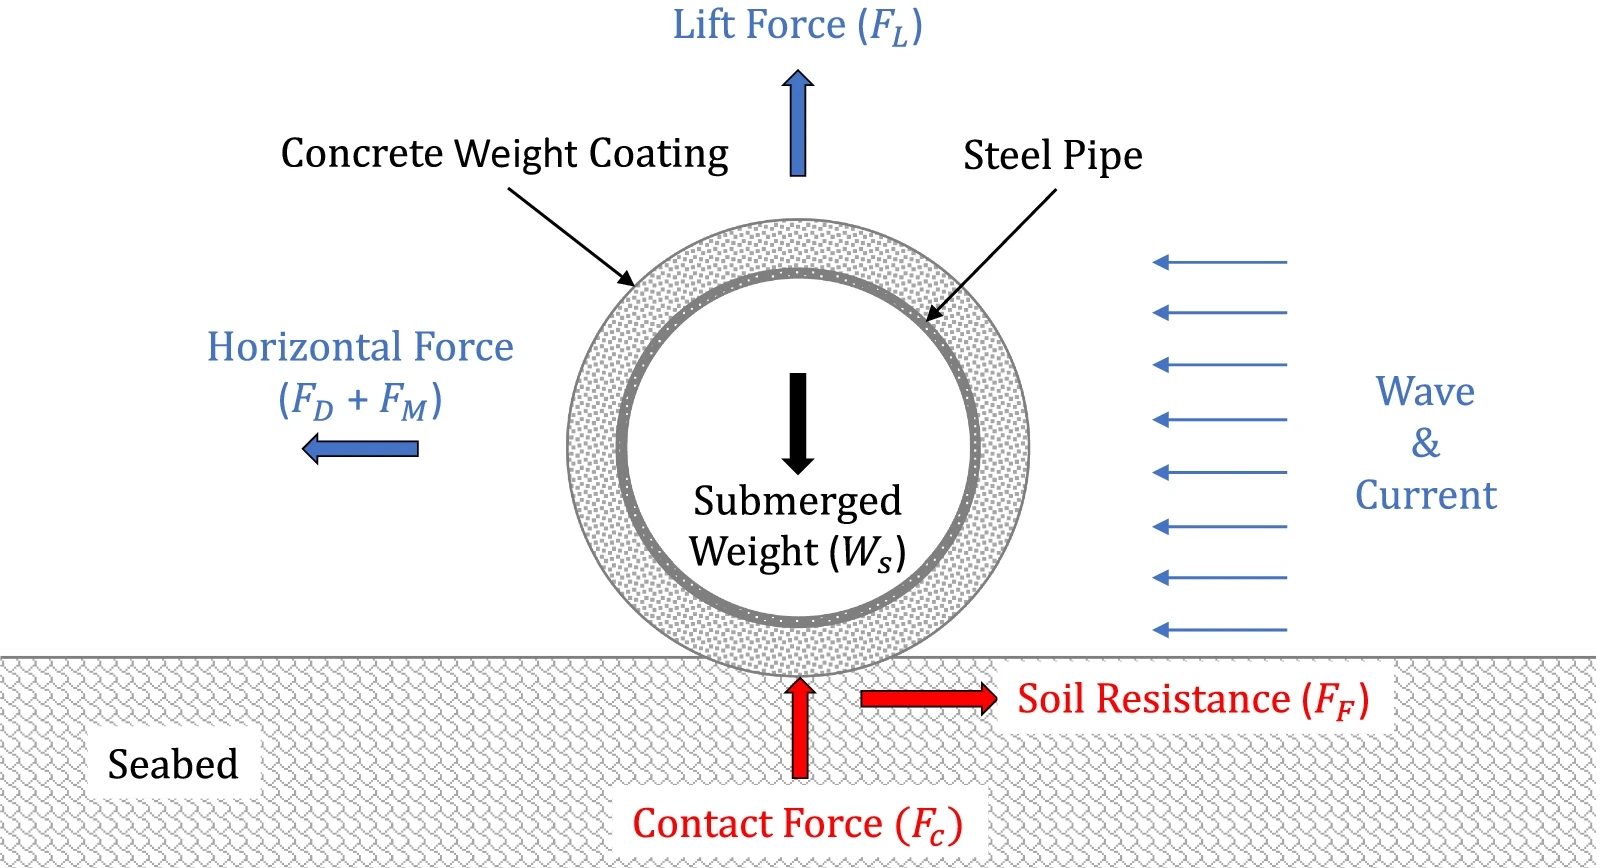
\includegraphics[width = 0.5\linewidth]{PipelineForces.png}
    \caption{Forces affecting subsea pipeline laying on the seabed \cite{PipeForces}.}
    \label{fig:PipeForces}
\end{figure}

A cross section of an offshore pipeline would typically show four layers each playing a significant role in their operation and protection. These include a concrete weight coating (60-110mm), an anti-corrosion coating (4.2mm), a steel wall (23mm) which provides the structural integrity for high pressure operation and an internal flow coating (0.1mm). Typically cathodic protection is employed to protect against corrosion.

Although pipeline decommissioning is completed on a case-by-case basis, for the larger pipelines, such as the Trunklines considered in this project, pipelines are typically left on the seabed or buried \cite{OGAdecom}. 

\subsection{Diabatic Compressed Air Energy Storage (D-CAES)}
A simplified visual representation of a diabatic CAES system is presented in Figure \ref{fig:caestypes-d}, however the implementation and realisation of a practical system is more complex. The design limits of rotating turbo-machinery mean that the best overall system efficiency is only achieved through operating within limited windows of gas flowrates, pressures \textit{etc.} and through careful process heat management. A more practical implementation of a diabatic CAES system is presented in Figure \ref{fig:d-caes-diagram}.

\begin{figure}[b]
    \centering
    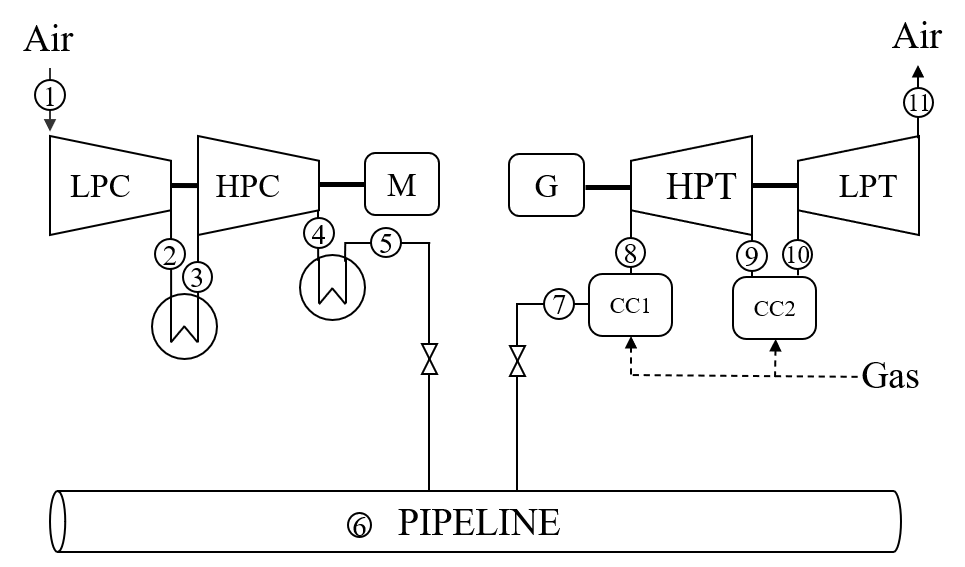
\includegraphics[width = 0.6\linewidth]{caes.png}
    \caption{Block diagram of proposed pipeline D-CAES schematic. M= Motor, G= Generator, LPC = Low pressure compressor, HPC= High pressure compressor, HPT= High pressure turbine, LPT= Low pressure turbine, CC= Combustion Chamber.
}
    \label{fig:d-caes-diagram}
\end{figure}

In the presented system, which has been implemented at the Huntof plant, during the charging phase, atmospheric air is compressed in two stages up to 74bar, each with a pressure ratio of 8.5, via a Low-Pressure Compressor (LPC) and a High-Pressure Compressor (HPC). Intercooling with a counterflow heat exchanger between the exit of the LPC and the entry to the HPC reduces the HPC’s compression work requirement. There is a possibility that the heat extracted at (2-3) and (4-5) could be stored and utilised as part of the discharge phase.

In the discharging phase, in order to maintain constant input conditions within the HPT, air is throttled to a constant 40 Bar. It is partially reheated by the stored heat before entering the first combustion chamber (CC1), where natural gas (or hydrogen) fuel source is ignited to increase the temperature of air entering the High-Pressure Turbine (HPT). The air is then expanded to 11 bar before entering the second combustion chamber (CC2) where it is reheated. The air is then expanded a final time in the Low-Pressure Turbine (LPT) to just above atmospheric pressure before leaving the system. 

Discharging is stopped when the pressure in the storage system reaches 30 bar since this is the design pressure of the HPT. Nevertheless, variable pressure turbines can also be utilised instead which could mean that the throttle stage is removed.

\subsection{Adiabatic Compressed Air Energy Storage (A-CAES)}
An adiabatic CAES system builds on the principle that both pressure and excess heat are generated in the compression phase \cite{BARBOUR2021102440}. The loss of heat represents a reduction in electrical conversion efficiency, rather than using natural gas (or hydrogen) to provide the heat during the discharging phase, the heat from the compression phase is recovered back to heat the expanding air. The principle is that an A-CAES system uses no gas and is thus more efficient.

A practical implementation of an adiabatic CAES system is presented in Figure \ref{fig:a-caes-diagram}. In this system, again based around a 70 bar peak pressure, three thermal stores, six heat exchangers, three compressors, three turbines and a pressurised gas storage vessel are used to construct a storage system. 

\begin{figure}[b]
    \centering
    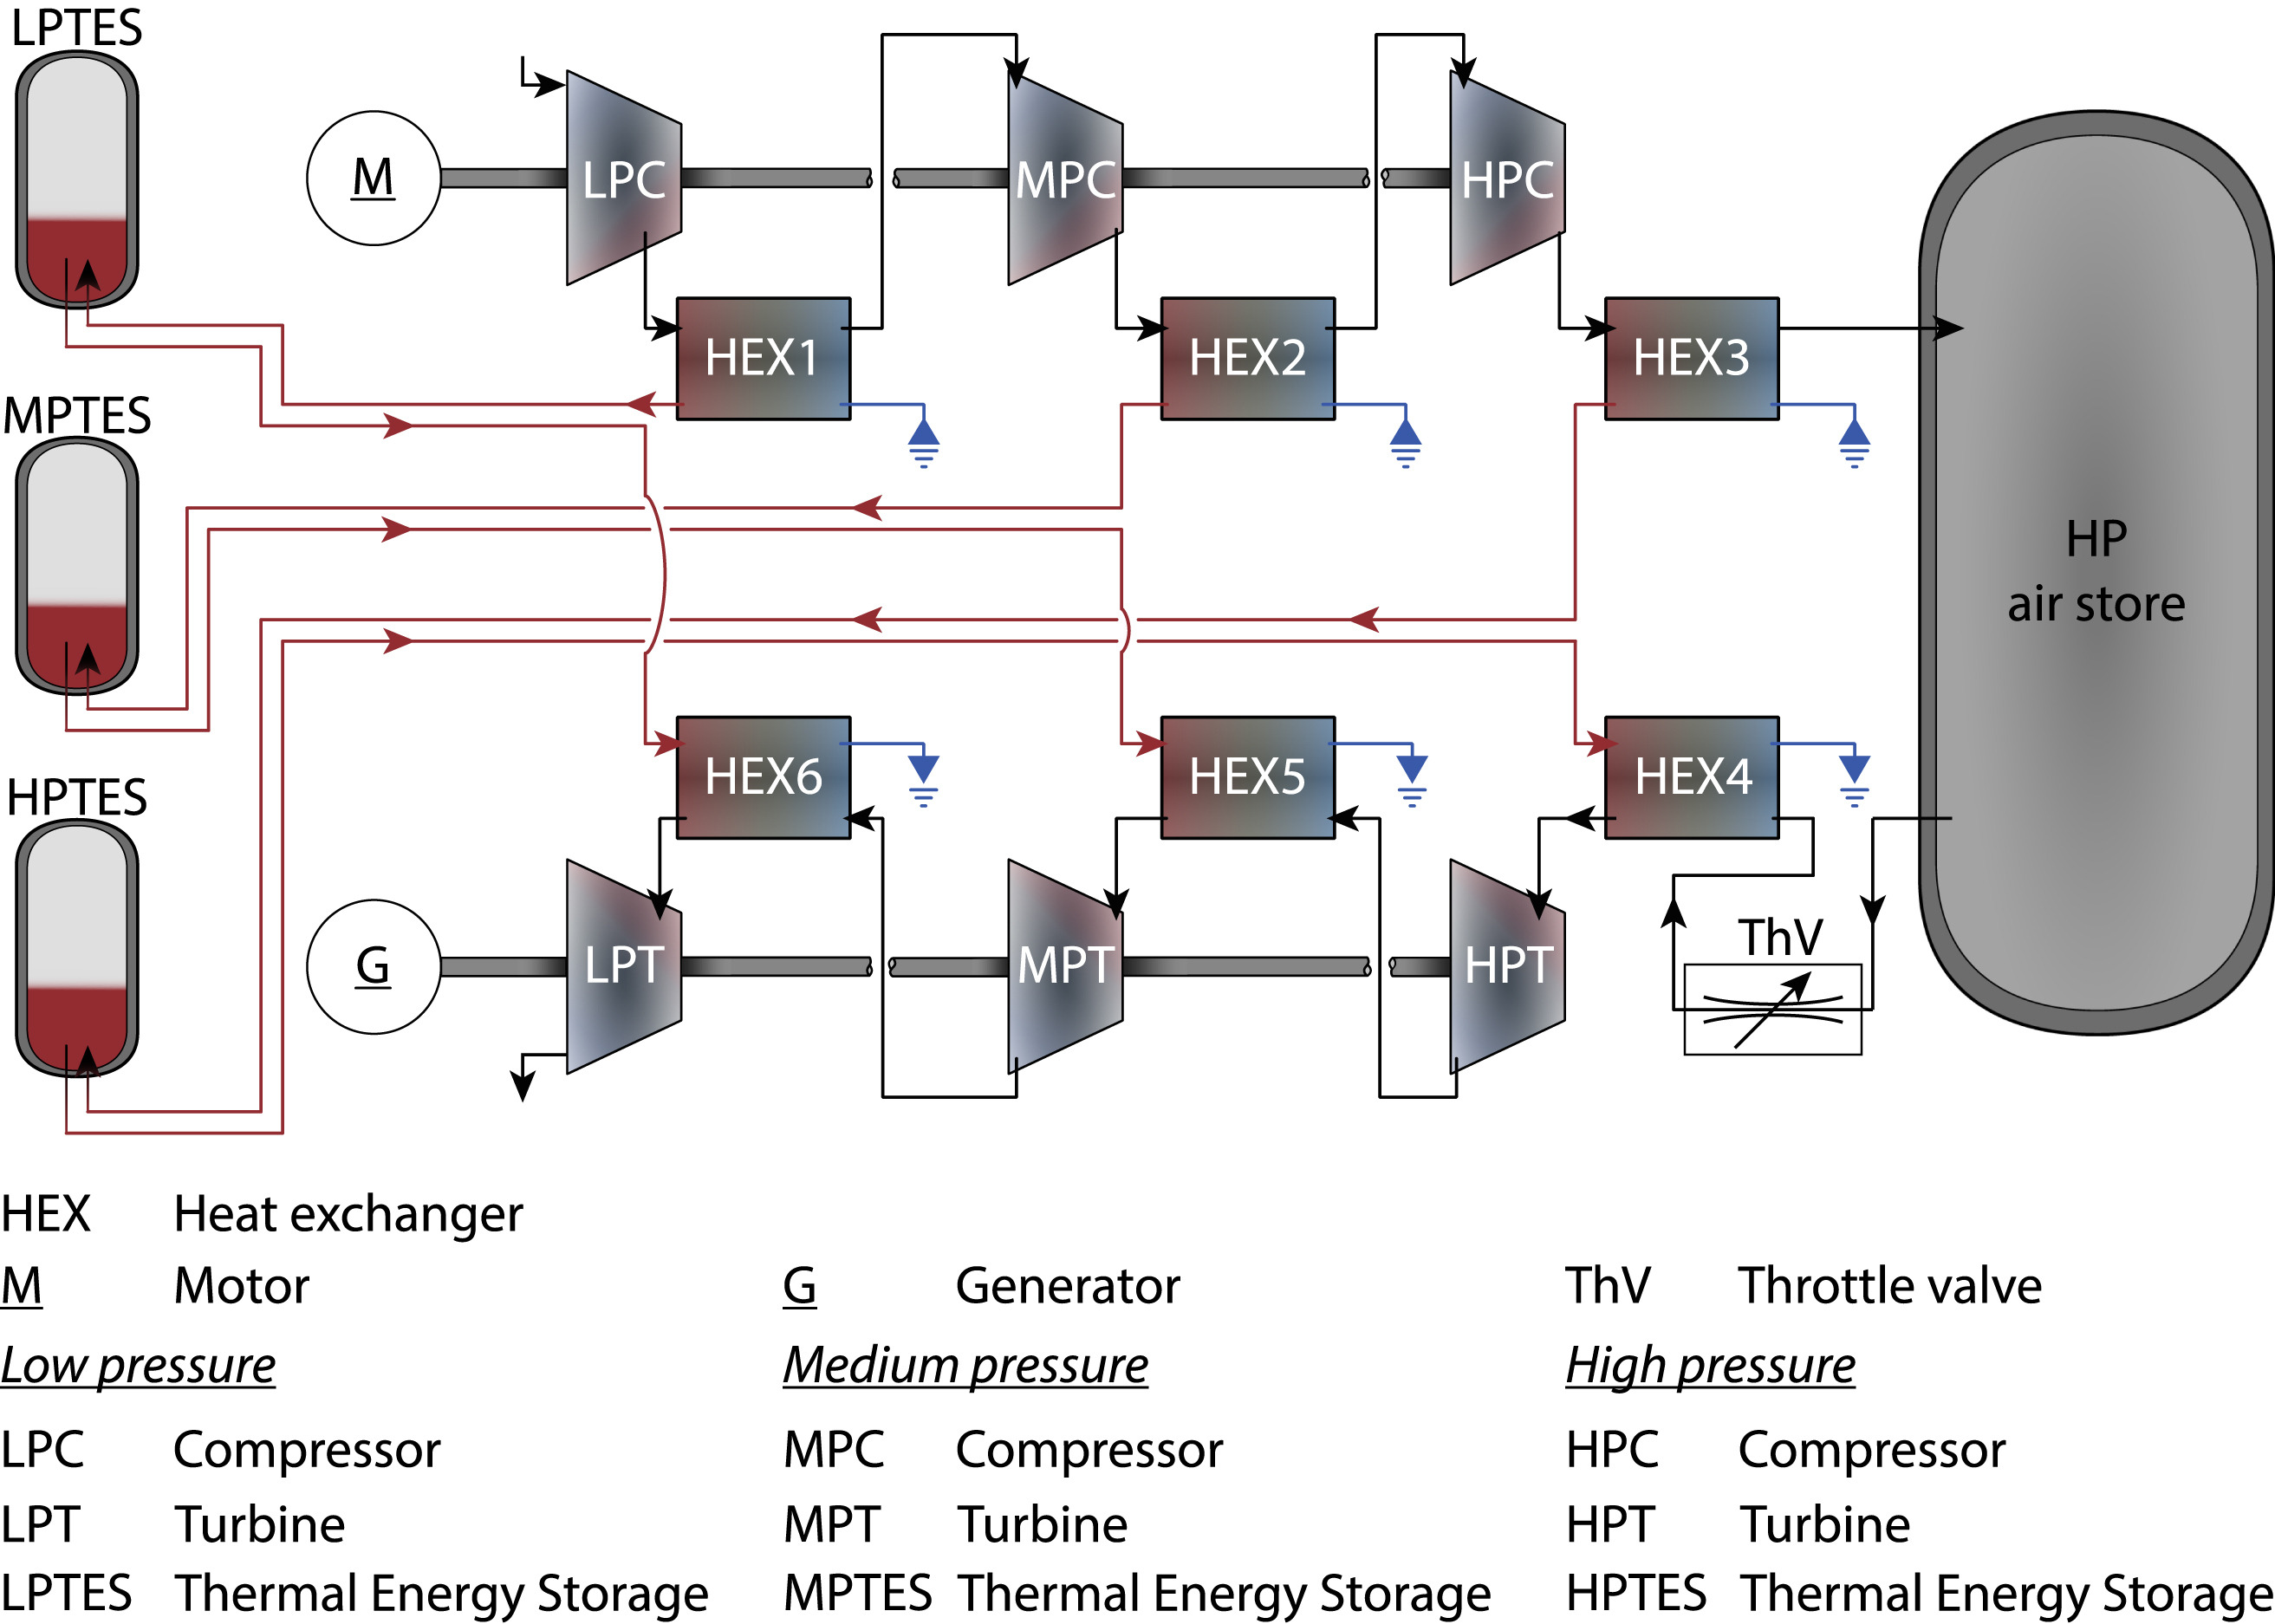
\includegraphics[width = 0.8\linewidth]{ACAES-StorageSystem.jpg}
    \caption{Block diagram of A-CAES schematic \cite{BARBOUR2021102440}.}
    \label{fig:a-caes-diagram}
\end{figure}

As observed, the system is notably more complex than D-CAES requiring three compression and expansion stages. Furthermore additional heat exchangers and thermal storage equipment is required. The principle is that such a system may be more efficient but this is offset by higher capital costs.

In the context of long-duration energy storage the requirement for equivalent thermal storage equipment may well be a barrier to deployment especially when the cumulative thermal losses from those stores may be significant.

\subsection{Parametric exploration of Pipeline Compressed Air Energy Storage (P-CAES)}
A validated thermodynamic model has been established using Thermolib-Simulink libaries and is detailed in the Appendix. The model was originally parameterised using data from a conventional D-CAES system coupled to geological storage. Pipelines are subject to a different set of constraints to those of geological storage and the following section explores some the key design parameters associated with a P-CAES storage system.

\subsubsection{Storage capacity of a pipeline}
This analysis considers that pipelines are cylindrical storage vessels of different lengths, inner diameters and maximum rated pressure. The thermodynamic model was used to determine the maximum storage capacity of the pipeline for a P-CAES system. In practice, it would be necessary to established a minimum rated pressure for the system. Largely this is associated with the compression/expansion train and its minimum pressure ratios. For simplicity and based on the Huntorf CAES Power plant, in the case applied, this has been fixed as 30 bar and as such this represents a minimum state-of-charge. Thus not all the energy storage in the gas compressed in the pipeline would be considered as recoverable. Hence if this is included in the analysis, the total Net Energy Storage Capacity per kilometre is determined and is presented in Figure \ref{fig:StoragePressure}.  

As presented, beyond the total length of a pipeline, the key sensitivities are the pipeline diameter and system maximum rated pressure. For context, pipelines in the North Sea would typically be in the 0.7-1.0m diameter range and rated at 80-150 bar. This would typically put their storage capacity in the sub 15 MWh/km range.

Nevertheless, for those systems where the maximum operating pressure were limited to less than say 100 bar, the 30 bar minimum could potentially be lowered further by utilising a different pressure ratio and compression/expansion train. 
  

\begin{figure}[h]
    \centering
    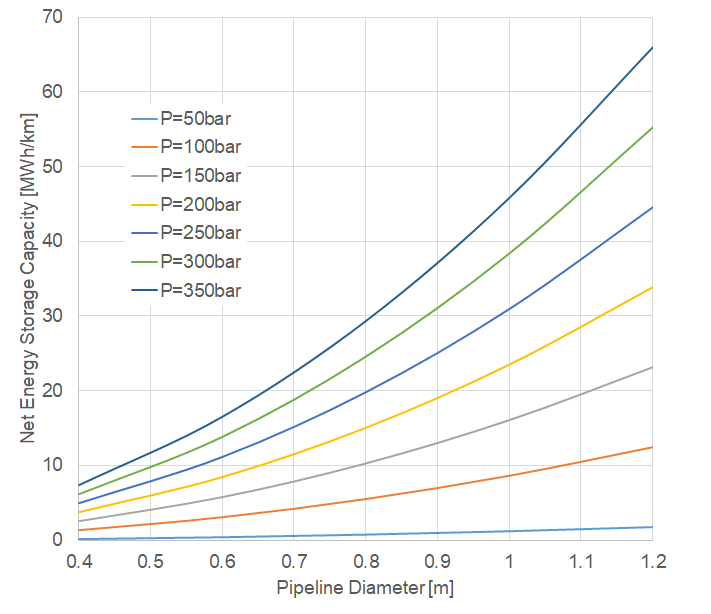
\includegraphics[width = 0.5\textwidth]{StoragePressure.png}
    \caption{Maximum net-storage capacity (MWh/km) per kilometre in a pipeline for various rated pressures based on a 40 bar minimum system pressure.}
    \label{fig:StoragePressure}
\end{figure}

\subsubsection{Storage system rated power}
\label{sec:RatedPower}
The specification of the CAES plant itself will be designed around its required maximum charging and discharge power. These design parameters will be established based around the demands of the local energy system, however there is no reason to suggest that maximum charging and discharge powers should be equal.

In principle, a CAES plant could be designed to a working maximum pressure of 100s of bar and at 100s MW. Hence, it is important to explore the influence of key design parameters and any potential limits imposed by the use of a pipeline itself. Ultimately one limit is the rate that pressurised gas can be pushed into the pipeline and any associated back pressures.

There are conflicting information regarding what is considered the maximum flowrate of a gas through a pipeline. Much of this appears to be borne out of the challenges of multi-phase fluids or fluids laden with debris which can lead to mechanical wear. Furthermore, as flowrates are increased as do the frictional losses associated with the interaction of the gas and vessel walls. As such, various figures for design flowrates have been identified for gas transmission, a 15 m/s flowrate has been identified by \cite{Walters2020}. This represents the average speed across a typical pipeline transporting gas from A to B. Of course, the proposed storage system is designed to have no net flow rate but a 15 m/s maximum has been imposed on charging rates to determine how much power this would consume. The results are presented in Figure \ref{fig:StoragePower} for a range of pipeline diameters and pressures.

The assumption of a 15 m/s maximum flowrate \cite{Walters2020} may well be too conservative for gas phase air with no net-flow across the pipeline volume. Other estimates or \textit{'rules of thumb'} might be in the 15-60 m/s range. The physics of the system mean that with a constant pipeline diameter, flowrates will be greatest next to the compression/expansion train and near zero at the far end of the pipeline. A figure suitable for the application under consideration needs to be identified. Hence, in order to understand the sensitivity of this as a limiting factor, the maximum charge powers are presented in Figure \ref{fig:StorageFlowrate}. In the 15-60 m/s range, we see a directly linear scale-up in the maximum charging power achievable from the system.

\begin{figure}[H]
\begin{subfigure}[h]{0.45\textwidth}
    \centering
    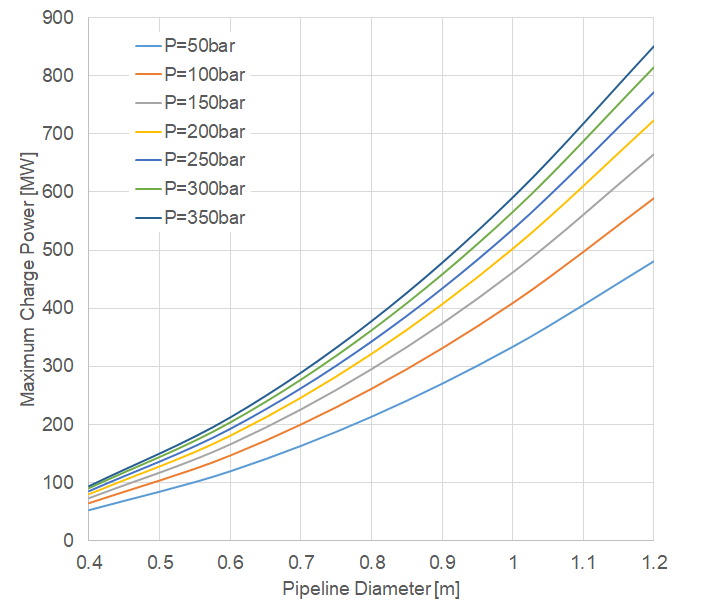
\includegraphics[width = 0.9\linewidth]{MaxCharge-Pipeline.png}
    \caption{Rated charging power for various pipeline diameters based on a 15 m/s flowrate limit \cite{Walters2020}.}
    \label{fig:StoragePower}
    \end{subfigure} 
\begin{subfigure}[h]{0.45\textwidth}
    \centering
    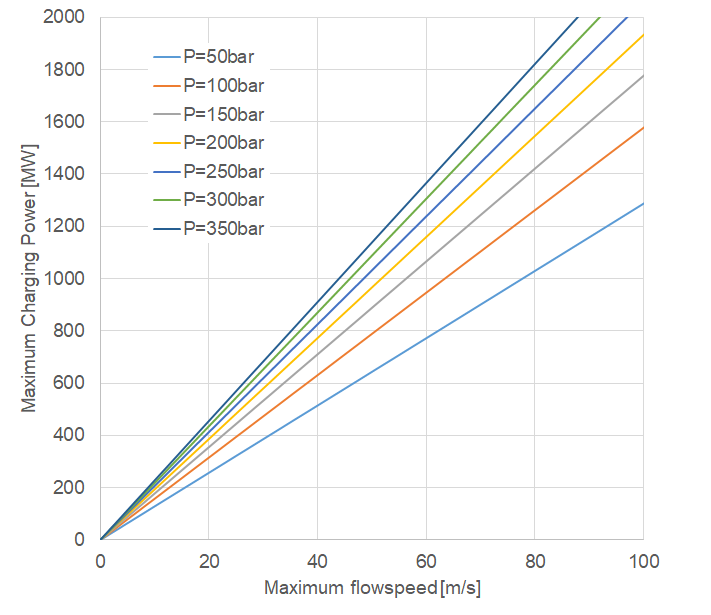
\includegraphics[width = 0.9\linewidth]{MaxCharge-Flowrate.png}
    \caption{Rated charging power for a range of final pressures based on maximum gas flow speed for a fixed pipeline diameter of 0.76m.}
    \label{fig:StorageFlowrate}
    \end{subfigure} 
    \caption{Approximate maximum rated charging power}
\end{figure}

The analysis carried out offers a yardstick as to the possible limits for charging power and maximum flow rates for the proposed solution. Following on from this, similar trends and sensitivities would also be expected for the maximum limits for discharging rates. 

\subsubsection{Storage system charging/discharging durations}
To illustrate the possible scale of a P-CAES energy storage system in terms of rated power and storage capacity, a range of potential systems are presented in Figure \ref{fig:StorageTimes}. Based around the utilisation of a 0.76m diameter and 100km long pipeline, a parametric sweep of potential systems are presented. Typically, the potential storage capacity is established by the system pressure with those with greater pressures capable of storing more energy. 

\begin{figure}[h]
    \centering
    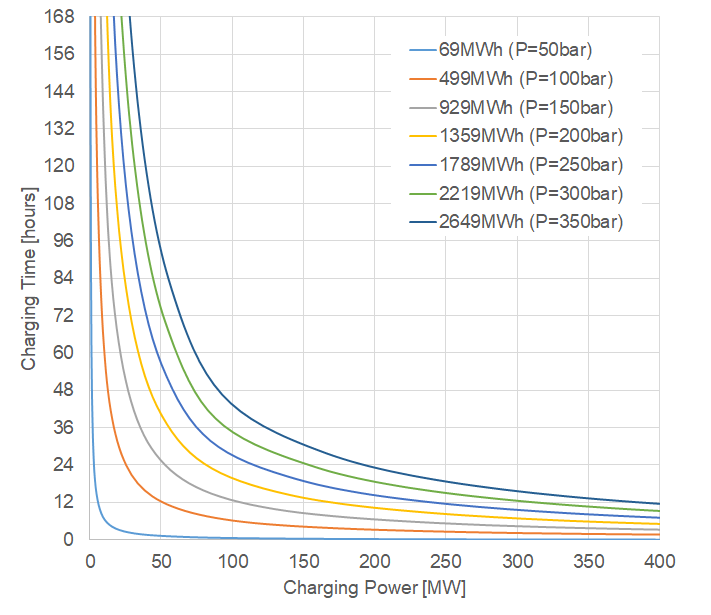
\includegraphics[width = 0.5\textwidth]{MaxCharge-Times.png}
    \caption{Approximate full system charging durations as a function of final system pressure and charging power for a 40 bar minimum, 0.76m diameter and 100km long pipeline.}
    \label{fig:StorageTimes}
\end{figure}

The various maximum rated charging power is then used to determine how long the system would take to charge at that particular power. Proportionally, a similar trend for discharging power would typically be expected. 

\subsection{Case studies of real-world pipelines around the UK's coastline}
\label{sec:systemsize}
The map of the UK presented in Figure \ref{fig:pipelinemap} presents an overview of many of the offshore (and onshore) pipelines. The thermodynamic model based on Huntof Plant was utilised to demonstrate the potential of CAES to be deployed in a pipeline application. Thus a 42 bar minimum and 72 bar maximum pressure system was used to estimate the rated storage capacity that each pipeline could potentially offer.

    %\todo{its not clear how this was determined - added an equation in the methods section}.
The total rated energy storage net capacity available for the 52 UK connected large pipelines can be estimated as 60.17 GWh, with a net storage capacity of 25.17 GWh. Figure \ref{fig:capacity} presents the rated storage capacity available at each pipeline landing. Figure \ref{fig:power} shows the maximum total turbine power by pipeline landing. The largest storage capacities are in St. Fergus followed by Easington and Bacton. 

Whilst it is not expected that all pipelines at each landing will be used for CAES, the scale of this opportunity is promising. Notably, the south section of the Langeled Pipeline which operates from the Sleipner riser to Easington offers the greatest potential for energy storage: a net capacity of 3.4 GWh. This is expected, since Langeled is the largest pipeline in operation. However, being a relatively new pipeline, transmitting a large proportion of the UK's gas imports, it is unlikely to be available for repurposing in the near future.

There are a series of decommissioned or nearly decommissioned pipelines which would enable a faster route to market. Such as BP's Miller to St Fergus gas pipeline which has already come out of operational use. When the Miller field ceased production in 2007, it was decided that the pipelines should be flushed of hydrocarbons and left in-situ. Full details of the decommissioning program are given in \cite{BP2011}. As a result of this, and a relatively short operational life, the pipeline is still in a suitable condition. The operation parameters adopted above would mean that Miller would offer a storage capacity of 700MWh at a power of up to 220MW.

The thermodynamic cycle used to analyse the storage potential used the operating conditions from the Huntorf plant. This was chosen as a good benchmark for comparing the system to previous CAES projects, and a large amount of literature was available for ease of comparison. However, the pipelines in question are designed to operate at up to 120-350 bar, considerably higher than CAES in salt caverns. Since a greater mass of air would be stored, operating at higher pressures, a larger storage potential may be expected with a higher round trip efficiency. The opportunities associated with a higher pressure system are explored in more detail in the following sections.

\begin{figure}[H]
    \centering
    \begin{subfigure}[h]{0.49\textwidth}
    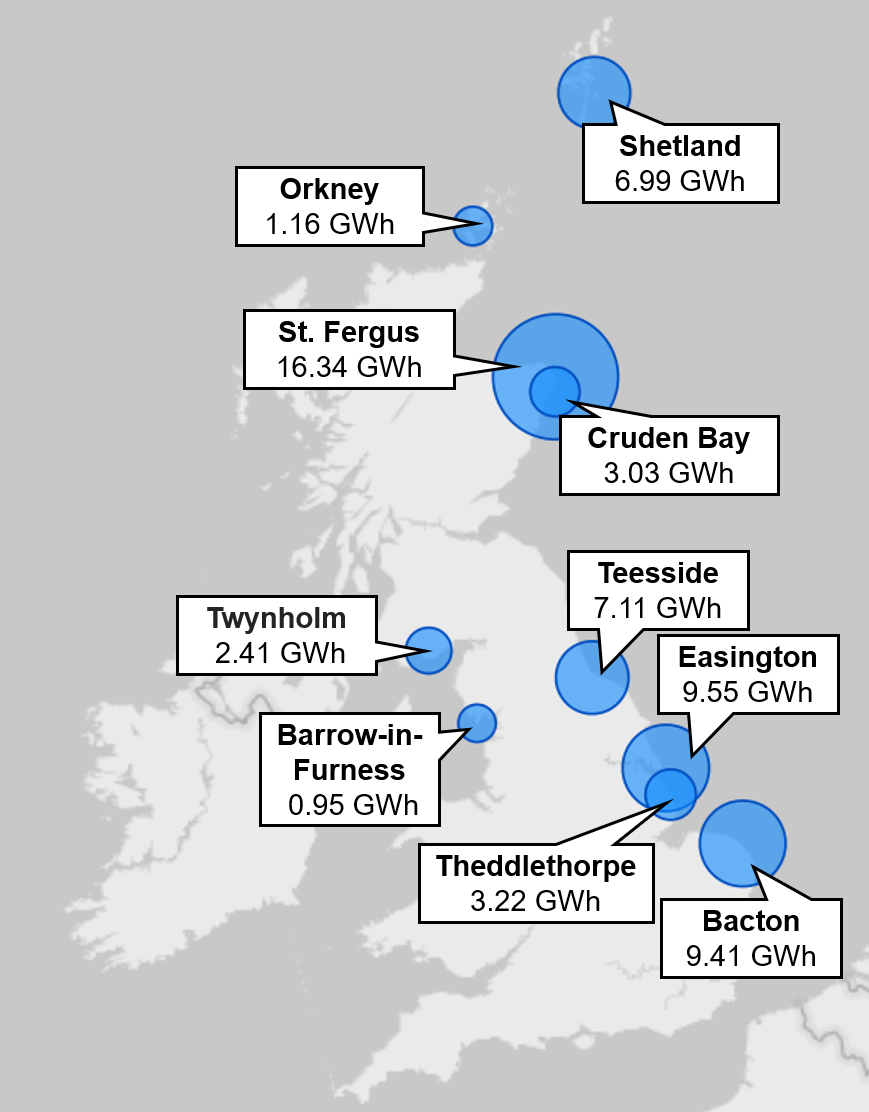
\includegraphics[width = 0.9\textwidth]{Capacity Map.png}
    \caption{Storage capacity by pipeline landing}
    \label{fig:capacity}
\end{subfigure}
\begin{subfigure}[h]{0.49\textwidth}
    \centering
    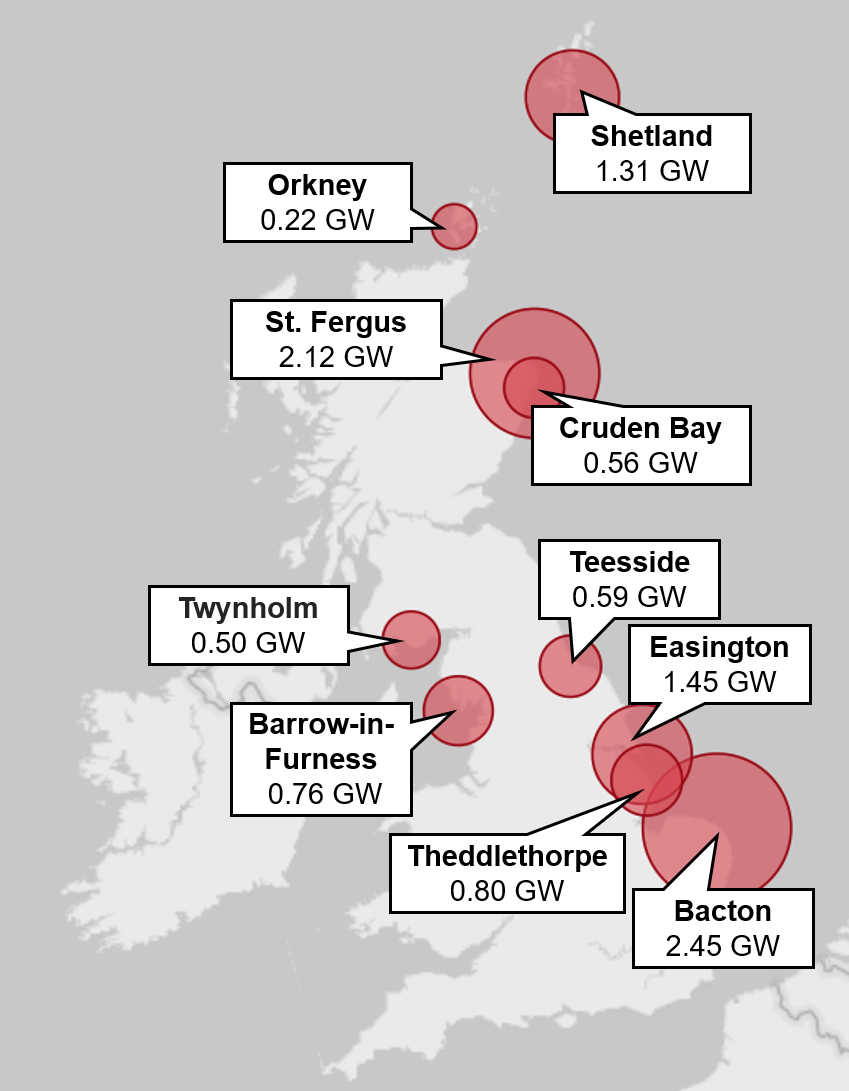
\includegraphics[width =0.9\textwidth]{Power Map.png}
    \caption{Power by pipeline landing}
    \label{fig:power}
    \end{subfigure}
    \caption{Total storage capacity and available power for pipelines connected to UK mainland}
\end{figure}    
    
\begin{figure}[H]    
\begin{subfigure}[h]{0.49\textwidth}
    \centering
    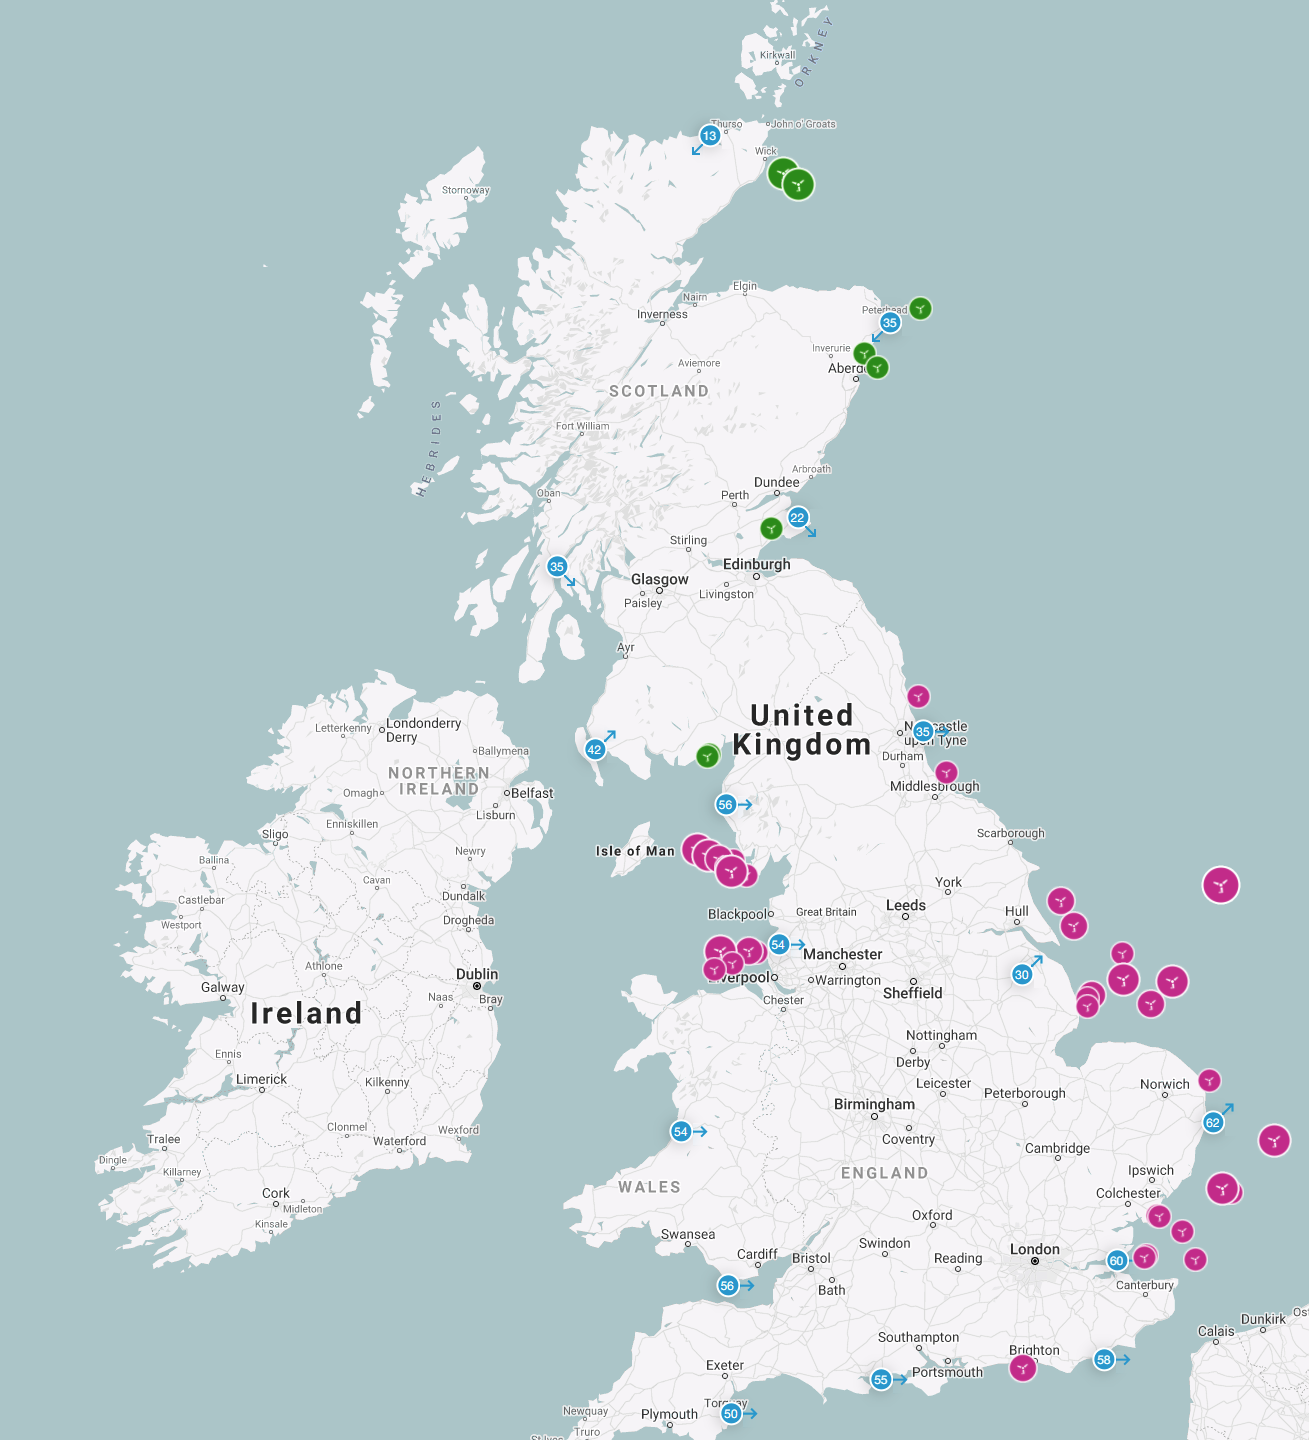
\includegraphics[width =0.9\textwidth]{UKwindfarms.png}
    \caption{UK offshore wind farm locations (Source: The Crown Estate).}
    \label{fig:wind}
    \end{subfigure}
\begin{subfigure}[h]{0.49\textwidth}
    \centering
    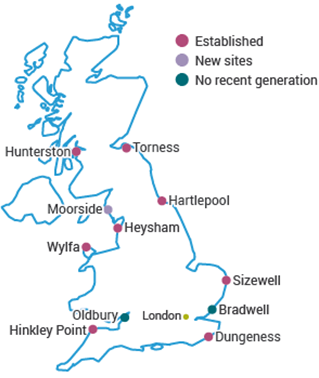
\includegraphics[width =0.9\textwidth]{uk-nuclear_thumb.png}
    \caption{UK current and planned and nuclear power locations (Source: World Nuclear Association).}
    \label{fig:nuclear}
    \end{subfigure}     
\begin{subfigure}[h]{0.49\textwidth}
    \centering
    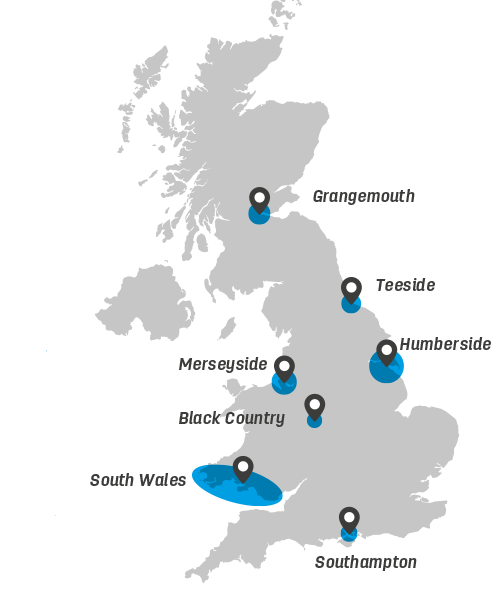
\includegraphics[width =0.9\textwidth]{UKDemandCentres.png}
    \caption{UK's major industrial energy demand centres}
    \label{fig:demand}
    \end{subfigure}    
\caption{The UK's wider energy infrastructure for supply and industrial energy demand}
\end{figure}

\subsection{Wider energy system and decarbonisation benefits}
\label{sec:energysystem}
As presented in Figure \ref{fig:wind}, the UK's offshore pipeline landing sites are in convenient proximity to many of its existing renewable wind power generation assets \cite{OGAmap}. Major wind farms such as Hornsea One (in operation) and Hornsea Two (planned) have a combined capacity of 2.4 GW, and both have onshore substations connecting them to the grid at Immingham which is 25 km to the Easington gas terminal and the location for a combined potential 9.55 GWh of storage. In addition to being the landing site for Norpipe and CATS, Teesside is also the planned landing for the 1.2 GW windfarm Doggers Bank C.

A similar picture can also be drawn around the UK's Nuclear power plants, Figure \ref{fig:nuclear}, with significant pipeline capacity with close proximity to reactors at Hartlepool, Sizewell, Heysham, Wylfa and Moorside.

Finally, the location of the available pipeline landing sites means that storage capacity can also be located close to many of the major industrial clusters in the UK. Historically, access to gas and ports has reduced manufacturing costs and as such local clusters have developed close to pipelines and local infrastructure. In particular, energy demand centres at sites such as Humberside, Teesside and Aberdeen would benefit from an abundance of local energy storage capacity. Furthermore, since the main storage capacity is held offshore, the landside footprint of such a plant would only be the CAES plant itself. This would dramatically assist with local congestion relief, resilience and assist with decarbonising these industrial clusters.
    
The installation of storage facilities can enable the local energy system to better manage bottlenecks and avoid the need for costly additional transmission infrastructure. As such, there is an immediate opportunity to support the growth of these assets and local electrical transmission management through complementing times of excess supply and re-balance demand with long-duration energy storage.
\subsection{Notional full-system design}

A summary of the technical parameters of a notional full-system design are set out in Table \ref{tab:FullSpecification}. The analysis which follows here has been carried out with the Miller to St. Fergus natural gas pipeline as an example. However as detailed in Section \ref{sec:systemsize}, the practical realities of the implementation of a P-CAES appear to be relatively similar across different sites and the analysis below could be considered as representative of many other opportunities across the UK. 

\begin{table}[h]
    \centering
    \begin{tabular}{lcc}
\hline
Discharging power capacity & {[}MW\textsubscript{e}{]} & 100  \\
Charging power capacity & {[}MW\textsubscript{e}{]} & 50 \\
Active pipeline length&  {[}m{]} & 240,000  \\
Pipeline diameter & {[}inches{]} & 30  \\
Maximum storage volume & {[}m\textsuperscript{3}{]} & 96,120  \\
Rated storage capacity & {[}MWh{]} & 3170  \\
Net storage capacity & {[}MWh{]} & 2623  \\
Maximum storage duration at full discharge & {[}hours{]} & 26.25  \\
Pressure range & {[}bar{]} & 30-174  \\
\hline
\end{tabular}
    \caption{P-CAES full-system specification based around the Miller Pipeline}
    \label{tab:FullSpecification}
\end{table}

\subsection{The Miller to St. Fergus offshore gas pipeline}

The notional full-system designed is based around utilising the Miller to St. Fergus natural gas pipeline presented in Figure \ref{fig:Miller}. This pipeline was commissioned in 1990 with a 25 year lifetime and is owned and operated by BP.

As presented in Table \ref{tab:FullSpecification}, the pipeline has a 240km length. It has an exposed and untrenched siting and an outside diameter of 30 inches. The pipeline has a maximum rated design pressure of 174 bar. 

\begin{figure}[h]
    \centering
    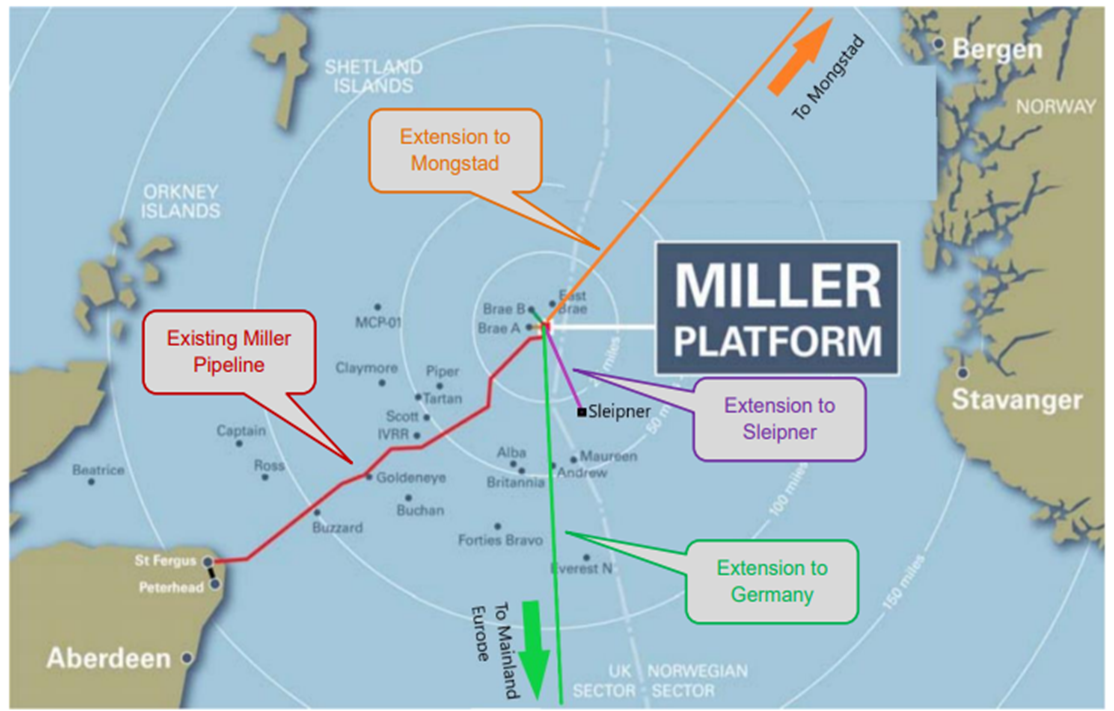
\includegraphics[width = 0.65\textwidth]{MillerPipeline.png}
    \caption{Map of the Miller Pipeline which connects St. Fergus to the Miller Platform.}
    \label{fig:Miller}
\end{figure}

\subsection{The St Fergus gas processing plant site}

The proposed location of the compressed air energy storage plant is in St Fergus and co-located with the St Fergus gas processing plant. As presented Figure \ref{fig:Miller}, the plant is near the village of St Fergus which is approximately 65 km (40 miles) north of Aberdeen and 11 km (7 miles) north of Peterhead, Scotland, UK. 

A schematic of the site is shown in Figure \ref{fig:StFergus}, the gas plant receives gas from the SEGAL (Shell Esso Gas and Associated Liquids) system. This includes wet gas transported from the Northern North Sea through the FLAGS (Far North Liquids and Associated Gas System) pipeline and from the Central North Sea through the Fulmar Gas Pipeline. It also receives gas from Norway through the Tampen pipeline, which connects the Norwegian gas transport system to the FLAGS system. 

\begin{figure}[h]
    \centering
    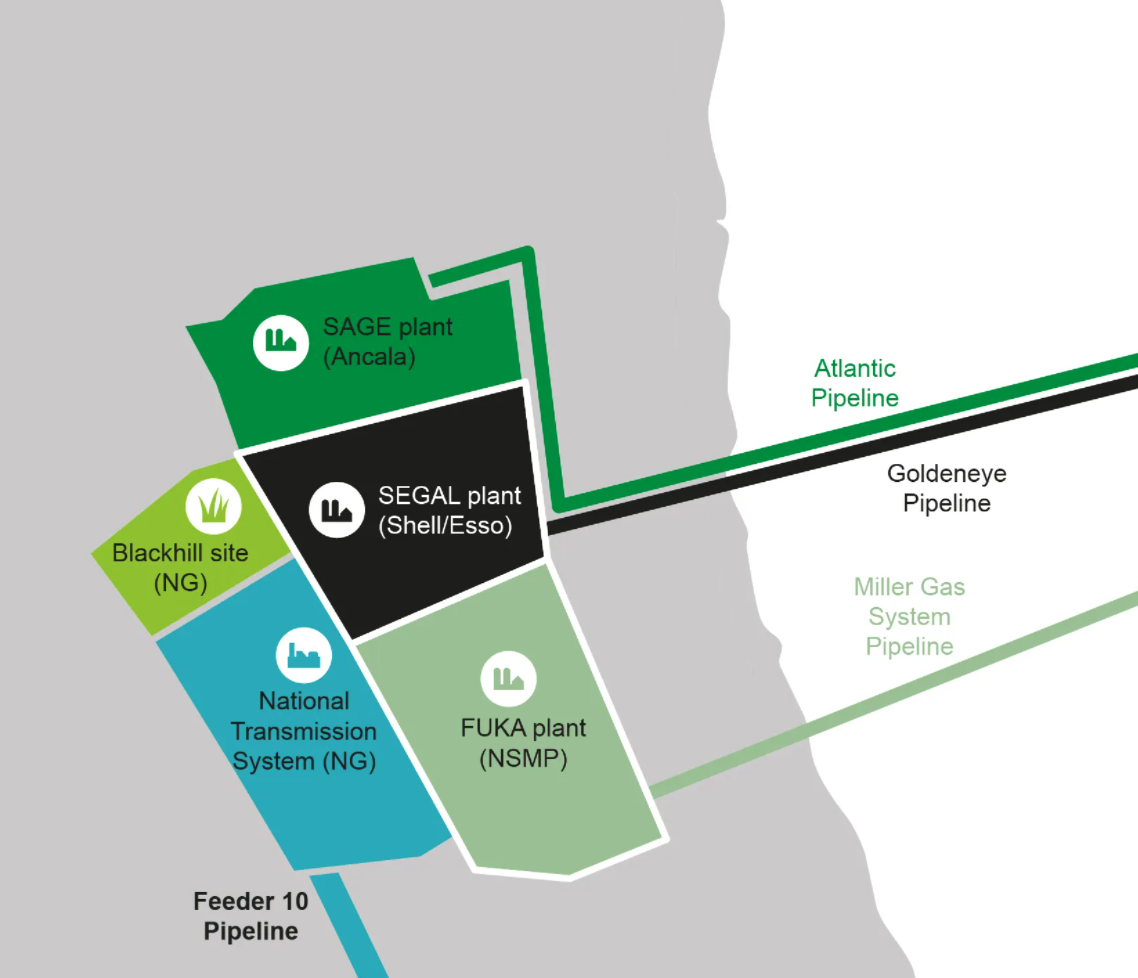
\includegraphics[width = 0.65\textwidth]{StFergusSchematic.png}
    \caption{Schematic of the St. Fergus gas processing plant}
    \label{fig:StFergus}
\end{figure}

The gas plant processes the natural gas as it is pumped ashore. Cryogenic processes are used to separate the hydrocarbon components. Methane gas is removed and delivered to National Grid for entry into the National gas Transmission System. The remaining hydrocarbons - Ethane, Butane, Propane and Gasoline, are pumped through an underground pipeline to the Shell Fife NGL plant for further processing.

As presented in the photographs shown in Figure \ref{fig:StFergusPhoto} and Figure \ref{fig:StFergusOS}, the site would be considered as remote/ rural and therefore would be considered to offer a significant amount of low-cost land. Additionally, since the objective here is to recommission existing assets, there maybe the opportunity of reducing plant installation costs by utilising the current foundations from the decommissioned gas processing facilities.  

The proposed powerplant specified in Figure \ref{tab:FullSpecification} has a footprint of around 20,200m\textsuperscript{2}, which corresponds to around 3-4 football pitches. A 50MW\textsubscript{e}/100MW\textsubscript{e} CAES powerplant would be of the approximate size of the red square in Figure \ref{fig:StFergusOS}. As shown in Figure \ref{fig:StFergus}, the Miller pipeline is the furthest south and locating the powerplant here would represent a viable opportunity in terms of space requirements and access to existing infrastructure for gas and electricity supply. For example, the site is a hub for natural gas processing with a national grid connection and is already served by a 132/11kV powerline which was upgraded in 2021. There are two 30MVA 132/11kV grid transformers at St Fergus Gas Station substation which is located 400m from the gas processing site.

\begin{figure}[h]
    \centering
    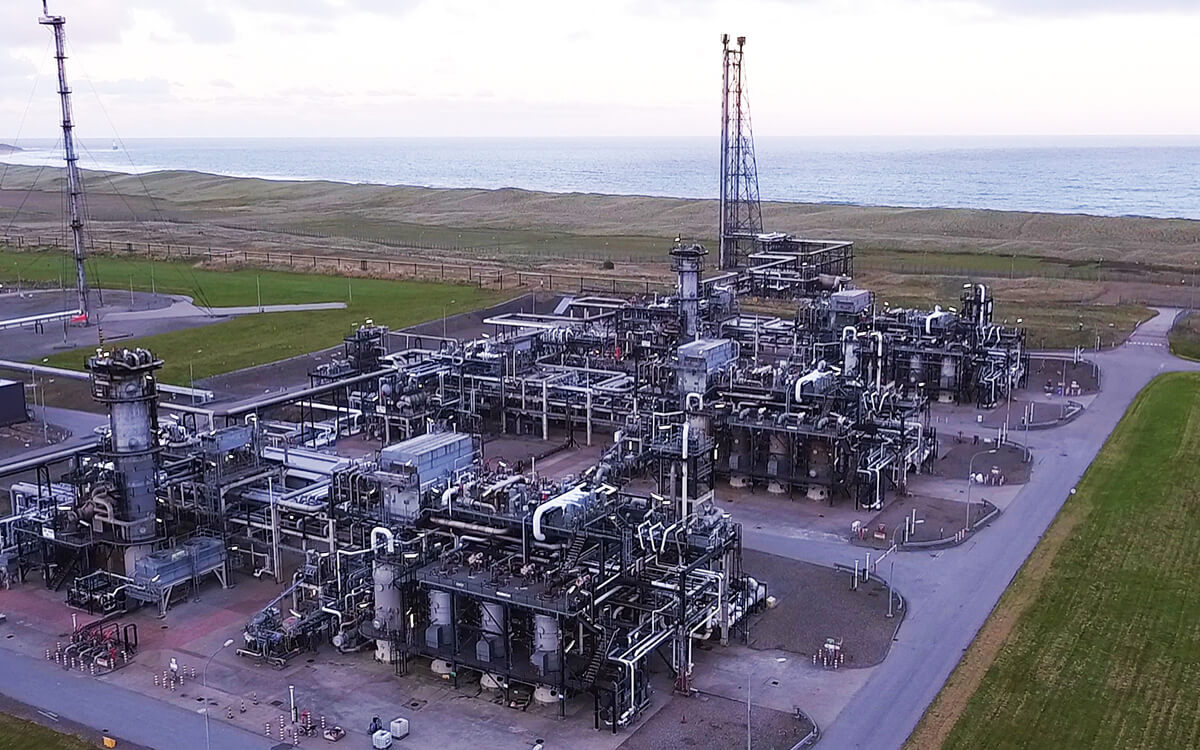
\includegraphics[width = 0.85\textwidth]{StFergusPhoto.png}
    \caption{Photograph of the St. Fergus gas processing plant}
    \label{fig:StFergusPhoto}
\end{figure}

\begin{figure}[h]
    \centering
    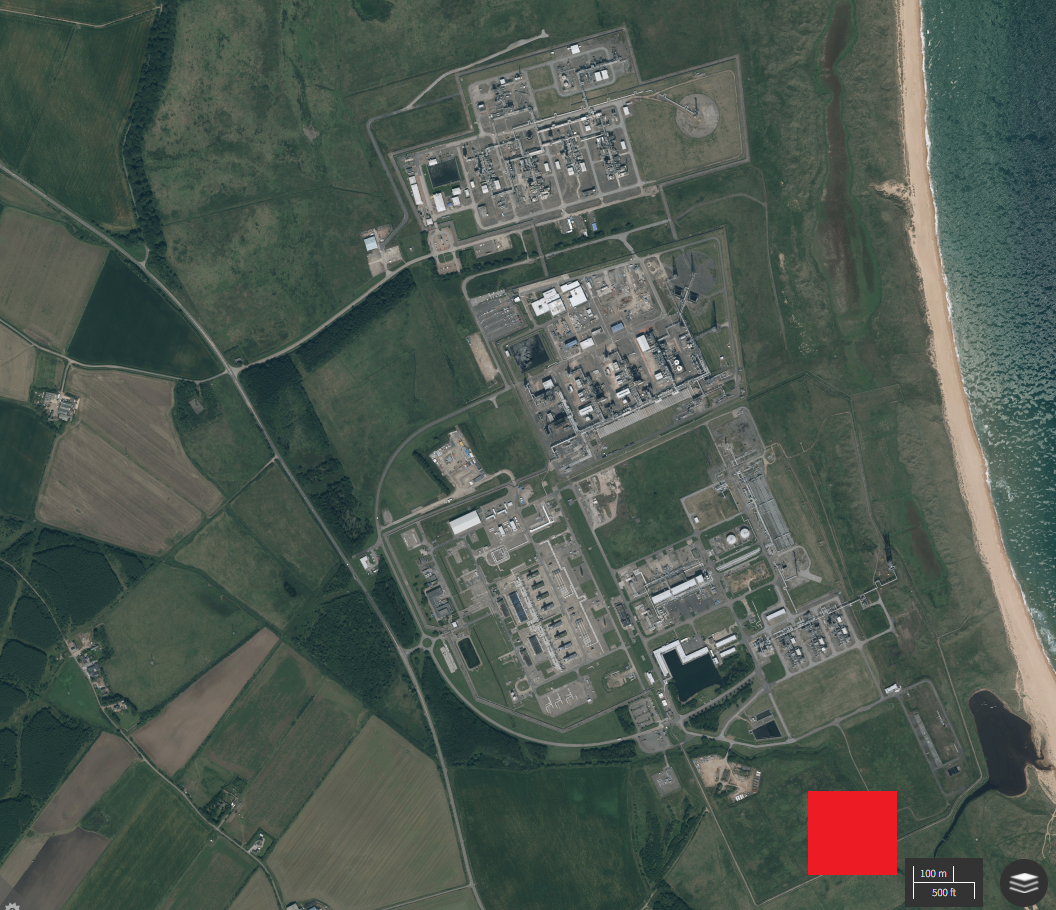
\includegraphics[width = 0.65\textwidth]{StFergusOS.png}
    \caption{Overhead photograph of the St. Fergus gas processing plant. The red square represents the size of the required 50MW\textsubscript{e}/100MW\textsubscript{e} powerplant relative to the site.}
    \label{fig:StFergusOS}
\end{figure}

\subsubsection{Access to intermittent renewable power supply}
\label{sec:MillerRES}
As presented in Figure \ref{fig:MillerWind}, the region around the St. Fergus gas processing plant has multiple potential offshore wind development opportunities which could be supported by the co-location of long-duration energy storage.

There is a case for performing a holistic analysis of the cumulative economic and energy system wide benefits that installing the system proposed in Table \ref{tab:FullSpecification} might have when co-developing these same offshore wind assets in the region. For example, corresponding onshore power network upgrades may not be as significant when inflexible peak/off-peak power demands can be supported by flexible storage.

\begin{figure}[h]
    \centering
    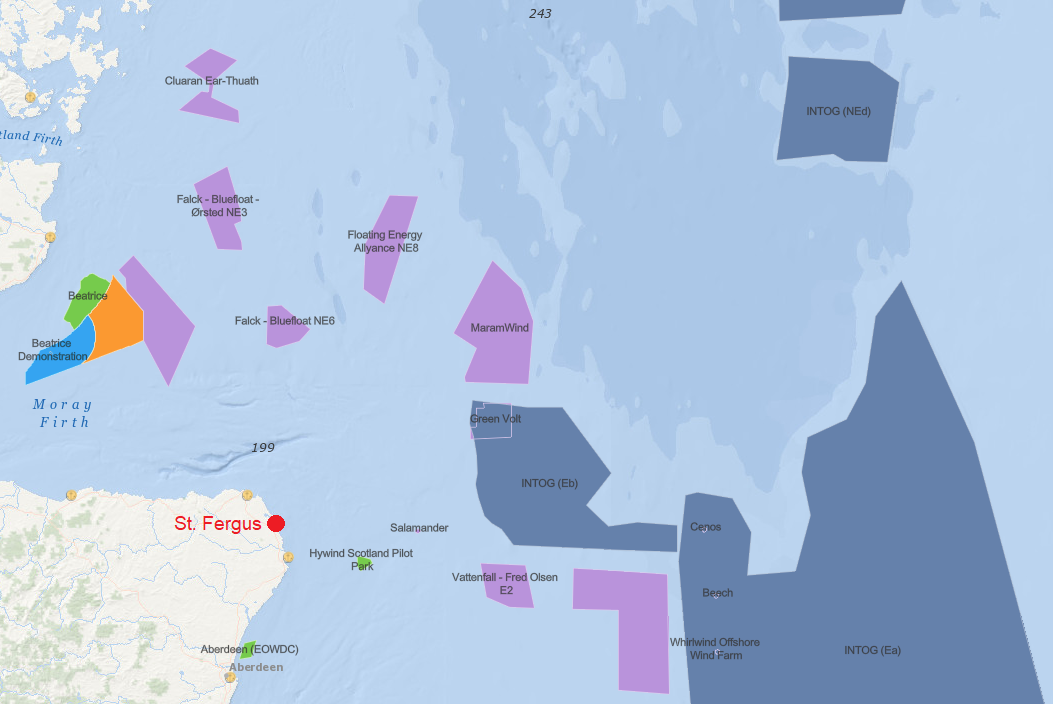
\includegraphics[width = 0.85\textwidth]{MillerWind.png}
    \caption{Offshore wind installations and potential sites close to the St. Fergus gas processing plant}
    \label{fig:MillerWind}
\end{figure}

\subsection{Overall system analysis}

When recommissioned as the storage medium in a P-CAES system, the pipeline would offer the corresponding storage capacities outlined in Table \ref{tab:FullSpecification}. 

\subsubsection{CAES powerplant}
\label{sec:CAESpowerplant}
With CAES the fundamental technology being employed, the rated system power for charging and discharging is independent from the rated storage capacity. In the proposed notional system design these have been scaled proportionally with the optimised long-duration energy storage systems presented by Hunter \textit{et al.} \cite{HUNTER20212077}, \textit{i.e.} discharging power is twice the charging power.
In principle, charging/discharging capacity can be added or removed as a retrofit as the UK market evolves to improve the cost effectiveness of operating a system.

The 1:2 charge:discharge power ratio is designed to best support a future and hypothetical net-zero energy system which is most likely to emerge in the United States. Nevertheless, in the absence of an equivalent analysis of the future UK market, it does offer insight into the premise that long duration storage systems are more profitable when taking advantage of a market short on renewable supply. However, as noted in Section \ref{sec:MillerRES}, a system designed and scaled to specifically complement wind power intermittent may well be the opportunity for the Miller pipeline. Under these circumstances, such a plant may well operate more cost effectively with a different charge:discharge ratio and corresponding maximum storage duration. In the absence of a detail scale-up plan for offshore wind in the region, for simplicity the 1:2 charge:discharge power ratio was retained.

A schematic of the proposed CAES powerplant is presented in Figure \ref{fig:SchamaticNotional}. This system is based upon a compressed air energy storage design offered by \textit{Siemens Energy}, which in itself is based on the experience of designing the McIntosh CAES Plant which has been operated since 1991.

\begin{figure}[h]
    \centering
    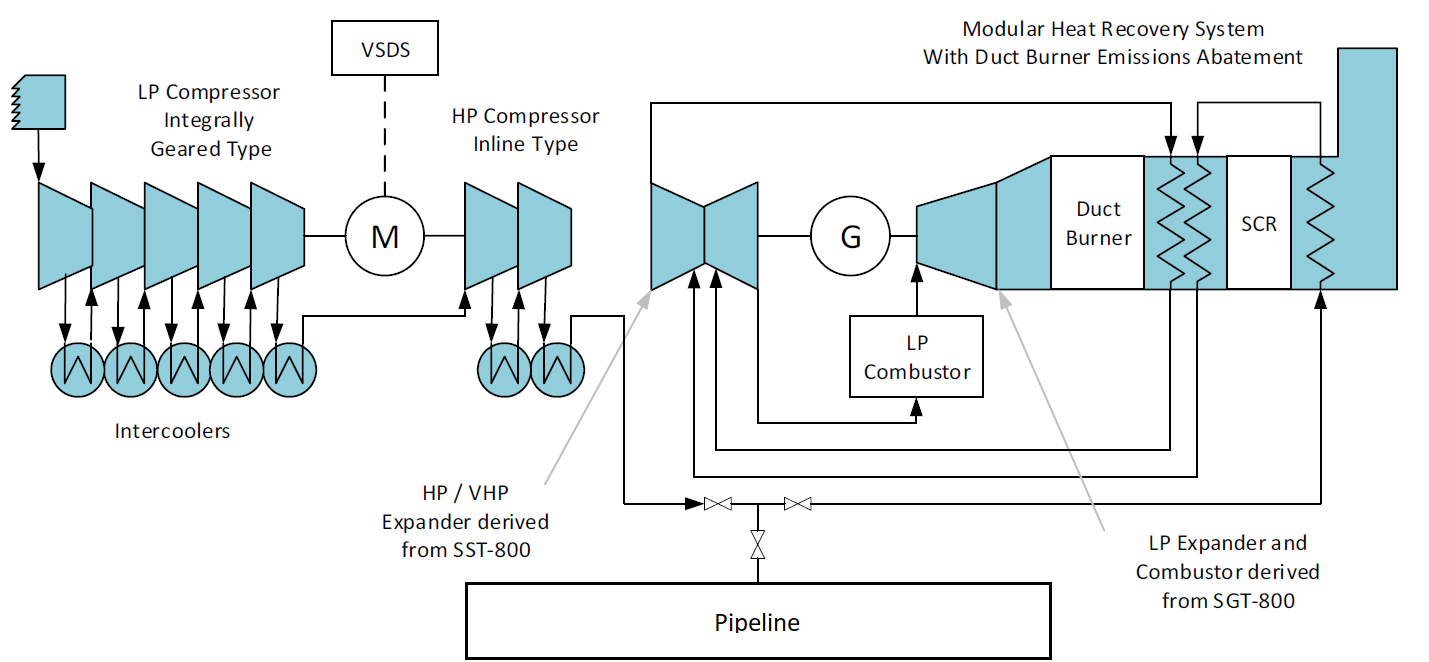
\includegraphics[width = 0.95\textwidth]{CAESPipeline-Siemens.png}
    \caption{Schematic of the planned notional P-CAES system.}
    \label{fig:SchamaticNotional}
\end{figure}

The design offered by \textit{Siemens Energy} is presented in Table \ref{tab:Siemens} with corresponding costs and components detailed. These data have been scaled (down) linearly to estimate the cost of the proposed CAES powerplant at St. Fergus. The same scaling has been applied to increase the pressure to a 174bar maximum.

\begin{table}[h]
    \centering
    \begin{tabular}{p{3cm} p{3cm} p{1.5cm} p{2cm}}
\hline
 & Unit & Cost (\$m (US)) & Uncertainty\\
 \hline
160MW expansion train & Siemens SST-800 and SGT-800 & 55 & 10\%\\
105MW compression train & Siemens DATUM and STC-GV & 35 & 10\%\\
Balance of plant & & 30 & 15\%\\
Construction & & 75 & 20\%\\
\hline
Total cost & & 195 & \\
\hline
\end{tabular}
    \caption{Siemens Energy CAES system design and costs. Each unit requires 5 acres of land.}
    \label{tab:Siemens}
\end{table}

The compression train is based upon a six-stage integrally geared low pressure
(LP) compressor followed by a two-stage inline type high pressure (HP) compressor. The compression stages are designed to be carried out at low-pressure (LP) using a DATUM unit (over 1,200 installed) and then at high-pressure (HP) by a STC-GV unit (over 2,000 installed). These can be scaled up to 125MW with a 105MW compression system costing \$35m.

The expansion train is based up a HP expander derived from Siemens SST-800
steam turbine (350 installations) and LP expander with dry low emission (DLE) combustion
system derived from Siemens SGT-800 gas turbine (130 installations). The system is integrated with an Selective Catalyst Reduction (SCR) technology to minimise NO$_x$ emissions. These can be scaled up to 160MW and 140MW respectively with a 160MW turbo-expansion system costing \$55m.

Discussions with \textit{Siemens Energy} indicate that the base system design and its costs can be scaled-up/down in terms of both power and upper pressure based on a linear-scaling model based on the required power. The parameters outlined in Table \ref{tab:Siemens} are for a circa. 70 bar

\subsubsection{Storage system recommissioning}

Recommissioning the Miller to St. Fergus natural gas pipeline means that up to 240km of offshore pipeline would be available for storing compressed air up to 174 bar. This corresponds to a storage volume of 96,120m\textsuperscript{3}. Based on a pressure range of 30 to 174 bar, this corresponds to up to 26.25 hours of storage capacity at 100MW\textsubscript{e}. 

The process of recommissioning a pipeline in relatively good condition would cost around £55/m. This means that the notional storage system has a Specific CAPEX (energy based) of approximately £4.13/kWh, which if compared broadly is the lowest of all non-chemical commonly reported forms of electricity energy storage \cite{Julch2015}. With this in mind, it therefore represents a solution which is very suitable for long duration energy storage where storage costs comprise a larger proportion of the overall system cost.   

\subsubsection{Estimation of notional energy storage system costs}

Based largely on data obtained (and scaled) from \textit{Siemens Energy}, an estimate of the capital costs of the proposed plant are detailed in Table \ref{tab:NotionalSystemCosts}.

\begin{table}[h]
    \centering
    \begin{tabular}{lcc}
\hline
 & Cost (£m (GBP)) & Uncertainty\\
 \hline
100MW expansion train  & 25.8 & 10\%\\
50MW compression train & 25.3 & 10\%\\
Balance of plant & 13.0 & 15\%\\
Construction & 32.0 & 20\%\\
Pipeline recommissioning & 13.2 & 20\%\\
\hline
Total cost & 109.3 & \\
\hline
\end{tabular}
    \caption{Approximate capital costing of a P-CAES plant utilising the Miller offshore pipeline}
    \label{tab:NotionalSystemCosts}
\end{table}

As presented, the total system costs would be at around £110m with most uncertainty on the main plant construction and pipeline recommissioning costs. As outlined above, the core components are also utilised in conventional power generation and have extended service histories and are designed to operate with a specific operational life in mind. As such, estimates for operating and fuel (gas and electricity) costs can be estimated based on how frequently the system will be used and return revenue. 

The levelised cost of electricity storage methodology based around the parameters set out in Section \ref{Sec:Counterfactual} means that the notional energy storage system presented in Table \ref{tab:NotionalSystemCosts} would offer a levelised cost of storage of £115.33/kWh. A full counterfactual analysis which compares the differences between different storage technologies is set out in Section \ref{Sec:Counterfactual}. On balance, it is likely that the solution proposed offers the maximum economic value for an investment in long-duration storage.

In addition, as noted in Section \ref{sec:MillerRES}, the installation of the system may reduce the need for more costly local upgrades of local electrical power lines and infrastructure. 

Another opportunity to note are those associated with the co-location of the plant alongside a major gas processing plant. In both the CAES and gas processing plants engineers will be managing processes which require the utilisation and loss of high amounts of thermal energy in the form of low-grade heat or cooling. In principle, there is the potential of symbiotic utilisation, storage and management of these losses across both systems. 

\subsection{Ability for future scale-up}

The ability for future scale-up has been set out in terms of potential locations and the technology, installation and manufacturing.

\subsection{Potential locations for UK deployment}
As presented in Section \ref{sec:systemsize}, with the principle that the limit on location is largely associated with the availability of pipelines, P-CAES systems can be deployed widely across the UK. Examples are set out in Figure \ref{fig:capacity} and \ref{fig:power} based on a conservative 70 bar maximum pipeline rated pressure.

Each site has its own limits for scale-up in terms of the available pipeline diameter, length, its current status (in use or not) and its condition. However in the main, each site appears to already be electricity and gas network connected and well integrated into existing infrastructure. A full site techno-economic evaluation would need to be carried out to evaluate the economic, regulatory and technical viability of re-commissioning each pipeline for redeploying as a storage medium of a P-CAES system.

\subsubsection{Technology, installation and manufacturing}
The core technology which underpins CAES systems is based upon the same global and multinational engineering and manufacturing base which has delivered high-efficiency, MW- to GW-scale power fossil fuel power generation machinery including gas turbines, industrial compressors, heat exchangers and electrical machines. Furthermore the offshore sector is experienced in the safe handling of high pressure gases and maintaining engineering assets offshore. 

\section{Economic Analysis}
\label{Sec:Counterfactual}
The overall system economic and costing analysis is presented in this section. It has been separated into the fundamental costing of each of the powerplant and pipeline components, the operating costs, \textit{etc.} then an evaluation of revenue models, investment and project lifetime costs.

\subsection{CAES powerplant costs}
As noted in previous sections, there are a number of deployments of CAES and the technology builds directly upon the service histories of hundreds of installations of the corresponding sub-components (compressors and turboexpanders). As such, the likely system costs, operating lifetimes and costs come with a relatively high level of confidence.

\subsubsection{Capital expenditure}
Estimates of the Capital Expenditure (CAPEX) for the powerplant is based on the forecasted cost for the compression and turbine systems obtained from a linear shape function. The CAPEX of the powerplant includes the cost of the main components, balance of plant and the construction of the site.

The analysis carried out builds upon findings published previously in the public domain, notably in \cite{Julch2015} where the LCOS approach was applied to D-CAES and A-CAES. In these kinds of techno-economic analysis, the cost of the compression and turbine systems are generally considered in terms of the cost of the charging/discharging system or the power-based CAPEX.

When corrected to 2022 Great British Pounds, Julch \textit{et al.} \cite{Julch2015} estimated that the charging system would cost 188-308 £/kW (220-340 €/kW (2015)) and 325-531 £/kW (380-620 €/kW (2015)) respectively. They also defined the discharging system would cost 196-325 £/kW (230-380 €/kW (2015)) and 196-309 £/kW (230-360 €/kW) respectively. Similarly, the work of Schmidt \textit{et al.} \cite{SCHMIDT201981} defined the whole charging/discharging system of a CAES would cost 672 £/kW (871 \$/kW (2015)).

In 2021, a comprehensive analysis of various long duration storage systems carried out by Hunter \textit{et al.} \cite{HUNTER20212077} defined the cost as 381 £/kW (507 \$/kW) for the charging system and 569 £/kW (759 \$/kW) for the discharging system component.

Finally, the project has also engaged with \textit{Siemens Energy} who have provided costing for a 105MW compression and 160MW expansion train D-CAES system. When presented in the same terms as presented above, these would correspond to be 386 £/kW for the charging system and 437 £/kW for the discharge system.  

The various costing estimates \cite{HUNTER20212077} \cite{Julch2015} \cite{SCHMIDT201981}, have been carried out assuming to have a financial lifetime of 30 years \cite{HUNTER20212077} and efficiencies of 55\% and 70\% for D-CAES and A-CAES respectively.

These cases appear to show a range of potential costs for D-CAES with a range of 188-386 £/kW for the charging system and 196-596 £/kW for the discharging system. Many of the analysis carried out are based on systems with differing rated powers and other factors. Nevertheless, the general trend is that the compression stage is more expensive than the expansion stage. 

Table \ref{tab:specCAPEX} shows the specific component costs which have yielded from this analysis. It is recognised that there are uncertainties on cost and as such three scenarios have been put forward. These are defined as:

\begin{enumerate}
  \item \textbf{An optimistic scenario:} Based on the lowest costs reported or a easier implementation than generally anticipated.
  \item \textbf{A median scenario:} Based on the costs reported the team by \textit{Siemens Energy} but also recognising that these came with a 10-20\% range of uncertainty and that there are other vendors for key capital assets such as the compressors/expanders which may be more cost competitive.
  \item \textbf{A pessimistic scenario:} Based on the highest costs reported or a more challenging implementation than generally anticipated.
\end{enumerate}

\begin{table}[h]
    \centering
    \begin{tabular}{p{3cm}cccc}
\hline
 & Unit & Optimistic & Median & Pessimistic \\ \hline
Charging system CAPEX & £/kW & 188 & 287 & 386 \\
Discharging system CAPEX & £/kW & 196 & 396 & 596 \\ 
Charging/ discharging system OPEX & £/kW/year & 10.11 & 10.11 & 10.11 \\
Pipeline recommissioning CAPEX & £/m & 0 & 55 & 226 \\
Pipeline OPEX & £/m /year& 3.2 & 7.62 & 15.0 \\
\hline

\end{tabular}
    \caption{Specific CAPEX and OPEX for a D-CAES Powerplant}
    \label{tab:specCAPEX}
\end{table}

\subsubsection{Operating expenditure}
The CAES powerplant operating expenditure (OPEX) are the sum of the costs accrued for day-to-day plant operation including routine maintenance.

The total CAES powerplant operating expenditure, $OPEX_t$ is presented in Equation \ref{OPEX}.

\begin{equation}
\begin{split}
        OPEX_t= & OPEX_p\left(\frac{P_C+P_T}{2}\right)+ OPEX_E\left(\frac{W_C+W_T}{2}\right) c_{st}\left(P_c+P_T\right) cyc +
        c_{el} W_C+{ c}_{NG} G_{cc} +c_{\mathrm{CO}_2} eq_{\mathrm{CO}_2} G_{CC}+ r_{ins} CAPEX 
    \label{OPEX}
\end{split}
\end{equation}

In this analysis, operating costs were split by power specific ($OPEX_p$), and energy specific ($OPEX_E$) costs of 10.11 £/kW multiplied by the average turbomachinery rated power, $P$. Also, a start-up cost of 0.015 £/kW \cite{Julch2015} was included for each cycle. The cost of electricity was 35.00 £/MWh, and natural gas was 8.2 £/MWh. Both were estimated in 2021 based on the average of the previous 48 months wholesale price provided by Ofgem \cite{OFGEMprices}. 

In addition, the \ce{CO2} certificate cost was 29 £/t\ce{CO2}e \cite{OFGEMprices} where the amount of \ce{CO2} produced by the system was determined by the greenhouse gas reporting conversion factor, 0.184 t\ce{CO2}e/MWh \cite{BEISCO2}.  

Finally, it was assumed that insurance would incur an annual cost of 0.5\% of the CAPEX \cite{Julch2015}.

\subsection{Pipeline costs}

\subsubsection{Capital expenditure}

For a conventional CAES powerplant, either underground caverns or free-standing pressure vessels are employed. For context, Mouli-Castillo \textit{et al.} estimated the specific cost of underground storage to be 0.32-3.58 £/kWh (\$0.42–4.71/kWh) \cite{Mouli-Castillo} and in 100 bar artificial free-standing compressed air storage vessels to be 420 £/kWh \cite{Chou}. 

For a pipeline, various cases have been considered for the CAPEX in line with the projected decommissioning costs for the North Sea pipelines. The OGUK publication \textit{‘Decommissioning Insights 2020’} \cite{OGUKdecom} provides the most up to date estimate into decommissioning activity, structured into key areas. The cost associated with pipeline decommissioning represents 3\% of the total budget, at £425 million. To bring some context to the analysis, estimates for the cost of full pipeline decommissioning are a significant expenditure and made by the owner or state depending on any liabilities. For example a Brazilian study estimated the cost to be 87.4 £/m \cite{Brazil}, or a US study of decommissioning in the Gulf of Mexico determined an average of 142 £/m \cite{KAISER2017167}.

In the case of recommissioning pipelines for use as a compressed air energy storage vessel, there are a number of factors which would impact upon the likely costs associated with redeployment. Typically when at the end of its specified operational life, a pipeline would still be expected to be in a relatively good condition. Its lifetime can be extended following a full inspection and recommissioning plan carried out by an accredited professional offshore pipeline engineering team. If the pipeline was well maintained, managed and is in good condition, recommissioning costs could be minimal.

Additional costs might come from the state of the pipeline and thus preventative repairs to specific lengths or sections may be required. If the pipeline were flooded with seawater, this water would normally need removal however unlike for gas/oil transmission, water accumulation in a CAES storage system would not be as significant especially if located far from the pipeline exit. Additionally for operation with a CAES plant, it is not completely necessary to entirely remove organic material. 

With the above uncertainties in mind, five scenarios are are considered for a comparison as below:

\begin{enumerate}
    \item `Simple' represents the best possible cost case, where the cost of recommissioning a pipeline has negligible capital expenditure and therefore incurs a cost of 0 £/m. All costs are within those of the annual operating costs of the pipeline.
    \item `Typical' assumes the recommissioning cost to be equal to the average specific recommissioning cost of 55 £/m \cite{OGUKdecom}.
    \item `Full-Recommissioning' takes the most conservative approach, with a recommissioning cost of 226 £/m \cite{OGUKdecom}, which is typical of flooded pipelines that would require significantly more work. 
    \item `New pipeline' - A new gas pipeline is also an option, albeit more expensive \cite{wiki} for example a modern offshore pipeline would expect to cost 1500-4000 £/m. There is some variance on these figures which depend on factors such as the diameter of the pipeline, its location, whether it is on- or off-shore \textit{etc.}. The Nord Stream pipeline reportedly cost 3000 £/m and this figure was adopted for the analysis.
    \item `Asset re-deployment' - As noted above, decommissioning has a significant cost to the pipeline owner of up to 142 £/m \cite{KAISER2017167}. Extending the lifetime of the asset means avoiding paying this cost by the pipeline owner/state. 

\end{enumerate}

\subsubsection{Operating expenditure}

Annual maintenance costs for off- and on-shore pipelines have been estimated by Chyong \textit{et al.} \cite{Chyong}. Their analysis was based around the offshore Nord Stream pipeline system, annual operating and maintenance costs were estimated to be 1\% and 1.5\% of the expected pipeline construction costs for offshore and onshore pipelines respectively. Based on the numbers above, this would correspond to 30 £/m per year. Others would put this as 3.204 £/m \cite {heddle2003economics} and 7.62 £/m (Crondall Energy).

\subsection{Proposed energy storage system}

The detailed specification used to explore the techno-economic potential of the P-CAES technology is set out in Table \ref{tab:technoecononomicspec}. The system has been specified to utilise the Miller offshore pipeline.

\begin{table}[h]
    \centering
    \begin{tabular}{lcc}
\hline
Discharging power capacity & {[}MW\textsubscript{e}{]} & 100  \\
Charging power capacity & {[}MW\textsubscript{e}{]} & 50 \\
Active pipeline length&  {[}m{]} & 240,000  \\
Pipeline diameter & {[}inches{]} & 30  \\
Maximum storage volume & {[}m\textsuperscript{3}{]} & 96,120  \\
Rated storage capacity & {[}MWh{]} & 3170  \\
Net storage capacity & {[}MWh{]} & 2623  \\
Maximum storage duration at full discharge & {[}hours{]} & 26.25  \\
Pressure range & {[}bar{]} & 30-174  \\
\hline
\end{tabular}
    \caption{P-CAES baseline specification}
    \label{tab:technoecononomicspec}
\end{table}

\subsubsection{Economic and utilisation parameters}

The system is expected to be operational from a revenue perspective (or discharging) for 15\% of the time on average over a year. This figure is based on a comprehensive technical analysis carried out by Hunter \textit{et al.} \cite{HUNTER20212077}, who explored the potential of various energy storage technologies in the US energy market in a potential net-zero scenario. They concluded that an energy storage technology with similar performance characteristics to a CAES system would be utilised at around 15\% based on the intermittency of a high renewable power energy mix and balancing against seasonal to daily consumer loads.

A less detailed by UK focused analysis by He, \textit{et al.} \cite{HE2021116097} built an optimal power flow analysis and optimisation model to determine the most appropriate specifications of various CAES systems. They estimated a figure of 19\% would be appropriate for CAES systems utilising underground storage sites.

The project’s interest rate, used as a discount factor in Equation \ref{LCOS} , was calculated, using Equation \ref{interest}, as 8.0\%. This incorporated the UK corporation tax $r_{tax}$ \cite{Tax2021}, the share of debt capital $s_{de}$, interest rate on debt capital $i_{de}$ and return on equity $i_{eq}$, which was adapted from \cite{Julch2015}.

\begin{theorem}
\begin{equation}
    i=\left(1-s_{de}\right) i_{eq}+s_{de} i_{de}\left(1-r_{tax}\right)\ 
    \label{interest}
\end{equation}
\end{theorem}

\subsection{Economic evaluation}
\label{sec:EconomicEvalution}
\subsubsection{Total plant capital costs}

The total plant capital costs are presented in Figure \ref{fig:CAPEX}. The analysis has been split into the pessimistic, median and optimistic costing scenarios. As presented in all scenarios, the most significant contribution to the total cost comes from those comprising the discharging component. However, with total costs ranging from £29m to £133m, there is significant uncertainty on the final system cost. The most significant variance from those aspects associated with the commissioning of the storage system itself. The cost of recommissioning a pipeline requires a specific technical evaluation of the integrity of the pipeline to be carried out to estimate the required level of work to be carried out. In practice, pipeline recommissioning is estimated to cost 0 - 226 £/m which in the baseline specification would correspond to 0 - 16.9 £/kWh of storage capacity.   

\begin{figure}
    \centering
    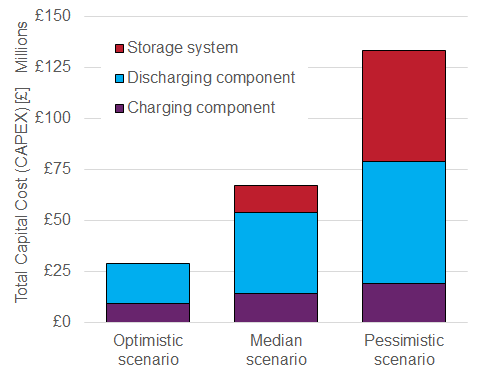
\includegraphics[width=0.5\linewidth]{P-CAES-CAPEX.png}
    \caption{Capital costs (CAPEX) of a P-CAES system designed at the baseline specification across the pessimistic, median and optimistic costing scenarios.}
    \label{fig:CAPEX}
\end{figure}

\subsubsection{Total plant operating costs}

The total costs of a P-CAES plant at the baseline specification at the median scenario would be £171m with the breakdown of those costs presented in Figure \ref{fig:TCCBreakdown}. More than 50\% of the lifetime costs are associated with the operation of the system, with more than 25\% from using electricity to charge the system.

\begin{figure}
    \centering
    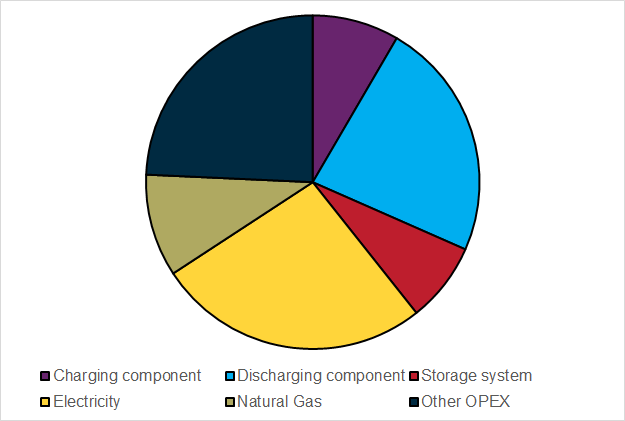
\includegraphics[width=0.5\linewidth]{P-CAES-TCCbreakdown.png}
    \caption{Total plant cost breakdown of a P-CAES system designed at the median baseline specification over a 25 year operational life.}
    \label{fig:TCCBreakdown}
\end{figure}

\subsubsection{Levelised Cost of Storage (LCOS)}

The Levelized Cost of Storage (LCOS) method was used to assess the financial feasibility of the proposed scenario and compare with previous cost models for CAES and other Electrical Energy Storage methods. LCOS assesses the total lifetime cost of a given storage system based upon the initial capital expenditure and the discounted sum of annual expenditures for the plants lifetime. This is then divided by the discounted total energy dissipated by the system. The annual cost is comprised of the operating cost (OPEX), reinvestments in the capital expenditure, and the cost of electricity consumed by the plant. At the end of the plant’s lifetime , any residual value the components hold is considered in $R_t$. The scenarios were analysed with a 30-year lifetime.  

\begin{theorem}
\begin{equation} LCOS\ =\frac{CAPEX+\sum_{t=1}^{t=n}\frac{A_t}{\left(1+i\right)^t}}{\sum_{t=1}^{t=n}\frac{W_{out}}{\left(1+i\right)^t}}
    \label{LCOS}
\end{equation}
where, \begin{equation} A_t=OPEX_t+CAPEX_{re,t}-R_t \end{equation}
\end{theorem}

Presented in Figure \ref{fig:LCOS} is the LCOS of a P-CAES system designed at the baseline specification across the pessimistic, median and optimistic costing scenarios. Based on a 35 £/MWh of electricity price, the three scenarios estimate a variance of 80 - 176 £/MWh and a mean of 115 £/MWh of electricity.

\begin{figure}
    \centering
    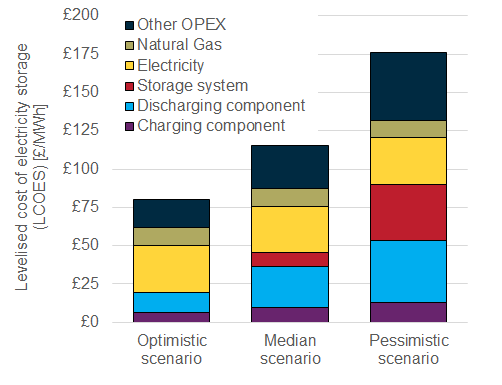
\includegraphics[width=0.5\linewidth]{P-CAES-LCOS.png}
    \caption{Levelised cost of electricity storage of a P-CAES system designed at the baseline specification across the pessimistic, median and optimistic costing scenarios.}
    \label{fig:LCOS}
\end{figure}

The most significant contributions to cost are those associated with the capital costs of the discharging component (approximately a third) and the operational costs associated with purchasing electricity to power the system (approximately a quarter).

\underline{Sensitivity to rated system power}: The influence of system rated charging and discharge power on LCOS is presented in Figure \ref{fig:LCOS-power}. As noted, the analysis has been carried out for the median baseline specification with different rates of charge/discharge, as the power ratings of the hardware used for compression and expansion are varied, the overall system costs are influenced proportionally. The analysis has retained a fixed discharging capital utilisation rate of 15\% which means that more revenue is generated as discharge power is increased, thus a lower LCOS is reported as the discharge power is increased. 

A parametric sweep of both charge/discharge power ratings for a fixed pipeline length has been performed to explore the dynamics of these relationships. Nevertheless the figure should be read with caution as some pairs of power ratings will not be technically feasible in practice, for example there are limits to the volume of air that can be stored in the system and obviously the compressor needs to be appropriately sized to replenish this supply prior to discharge.

However, the clear trend is that the most cost effective designs would minimise the rate power of the charging system and maximise the rated system power for discharge \textit{i.e.} the economics favours those systems with longer charges and shorter discharge durations.

\begin{figure}
    \centering
    \includegraphics[width=0.5\linewidth]{P-CAES-LCOS-power.png}
    \caption{Levelised cost of electricity storage of a P-CAES system designed at the median baseline specification for a range of maximum discharge powers. Various system charging powers have also been presented and are plotted as different lines. A fixed discharging capital utilisation rate of 15\% has been assumed.}
    \label{fig:LCOS-power}
\end{figure}

%\subsubsection{Sensitivity to final system pressure}

%The influence of system rated pressure on LCOS is presented in Figure \ref{fig:LCOS-Pressure}. A greater pressure, increases the total system storage capacity proportionally, for example a pipeline storing air at 50 bar is 4.62 kWh/m and 350 bar is 32.4 kWh/m with minimal additional CAPEX. 

%However, for a fixed system rated power and pipeline length, it is clear that increasing the system's maximum operational pressure increases the levelised cost of storage. The main contribution comes from the loss in efficiency. 

\begin{figure}
    \centering
    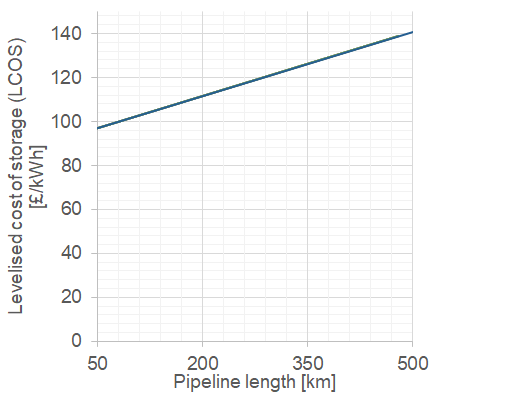
\includegraphics[width=0.5\linewidth]{P-CAES-LCOS-Pressure.png}
    \caption{Levelised cost of electricity storage of a P-CAES system designed at the baseline specification for a range of maximum system pressures and pipeline lengths.}
    \label{fig:LCOS-Pressure}
\end{figure}

\underline{Sensitivity to pipeline length}: The influence of pipeline length on LCOS is presented in Figure \ref{fig:LCOS-Pressure}. As pipeline length is increased so is the total system storage capacity alongside recommissioning and operating costs associated with the pipeline. The lower CAPEX and OPEX for a shorter pipeline means that it is more cost effective than a larger system albeit with a shorter duration for discharge. 

\underline{Sensitivity to utilisation of the system}: The LCOS analysis of the baseline specification assumes a discharging capital utilisation rate of 15\%, the sensitivity to this figure on LCOS is presented in Figure \ref{fig:LCOS-Utilisation}. For context, figures of 19 \% have been put forward for discharging capital utilisation rates for CAES systems operating in the UK for long-duration energy storage applications. This would represent a $<$10\% reduction in the overall LCOS for the solution.

\begin{figure}
    \centering
    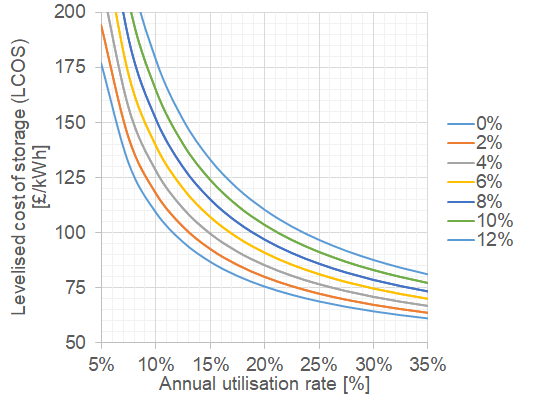
\includegraphics[width=0.5\linewidth]{P-CAES-LCOS-Utilisation.png}
    \caption{Levelised cost of electricity storage of a P-CAES system designed at the baseline specification for a range of capital (discharge) utilisation percentage rates. Lines represent different investor percentage rates of return.}
    \label{fig:LCOS-Utilisation}
\end{figure}

To achieve a discharging capital utilisation rate of 15\% - 25\%, then there must be a proportional and equivalent time expended in charging that same system albeit at a different rate. Hence, if exceeding the 25\% figure a larger compressor with a higher rated power may well be required and for it to be powered at times with greater electricity prices. 

\underline{Sensitivity to price of energy utilities}: An analysis of the relative contributions of the prices of natural gas and electricity are presented in Figure \ref{fig:LCOS-ElectricityGas}. It is expected that the system will take advantage of curtailed renewables, off-peak or reduced cost electricity prices and thus would be buying electricity at a lower costs (less than 50 £/kWh). The analysis generally shows a clear linear trend for prices in terms of both electricity and natural gas prices. 

\begin{figure}
    \centering
    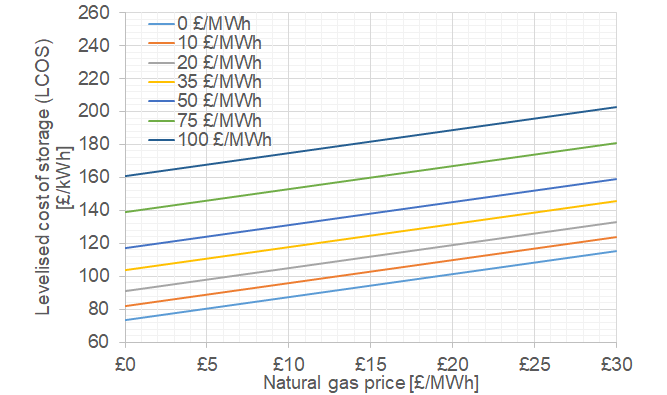
\includegraphics[width=0.5\linewidth]{P-CAES-LCOS-Utilities.png}
    \caption{Levelised cost of electricity storage of a P-CAES system designed at the baseline specification for a range of utilities rates.}
    \label{fig:LCOS-ElectricityGas}
\end{figure}

Net-zero power systems and the wider decarbonisation of society including heat, transport and heavy industry requires a transition away from natural gas and toward other energy carriers like hydrogen. Switching from hydrogen to natural gas represents one simple pathway which would make CAES net-zero compatible. Renewable electricity production combined with electrolysis is one scaleable pathway expected to yield so called 'green' hydrogen for utilisation across multiple sectors. If used as the primary energy source for re-heating in a CAES system, the main change to the system would be observed in minor changes to the combustion system on the discharge side and in terms of the relative cost of the gas. Bristow \textit{et al.} \cite{hydrogen2030015} have estimated future prices of green hydrogen production based on a renewable electricity price of 39.47 £/MWh to be upwards of around \$1.00/kg. This analysis determined that in a 2030-2050 time frame, an equivalent natural gas price of 22.80 £/MWh is a techno-economically viable price for green hydrogen. This combination would yield a LCOS of hydrogen fuelled P-CAES to be around 127 £/MWh. 

\subsection{Potential Revenue Models}

The previous sections have explored the Levelised Cost of Energy Storage (LCOS). However, there are a number of options which could incentivise investment and deployment of such large scale infrastructure but which can still fit within existing market frameworks. Some of the potential revenue models for funding an electricity storage plant are:

\begin{enumerate}
    \item Contracts for Difference (CfD)
    \item Income Cap \& Floor Model
    \item Regulatory Asset Base (RAB)
    \item Capacity Market (CM)
\end{enumerate}

\subsubsection{Contracts for Difference (CfD)}
The most common revenue model adopted for renewable electricity generation. A strike price for the electricity provided by the energy storage system is agreed via contract between the electrical power generator and the government/electricity network operator.

The mechanism aims to protect the investment from volatility in wholesale power prices. A strike price for the power is agreed which is honoured by government regardless of the wholesale price of power. With no temporal dimension, it is better suited for offering intermittent electricity supply to a network regardless of whether or not the network is in surplus or has a shortage of supply. 

Nevertheless, greater certainty can be brought forward using the principles of a CfD revenue model and it could be adopted for CAES applications but based on a 30 year time frame and with the following additions: 

\begin{enumerate}
    \item A fixed (peak) strike price for electricity provided to the network.
    \item A fixed (off-peak) electricity and gas price offered to the storage provider.
    \item An agreement to purchase electricity at the agreed strike price for a minimum number of hours per year (or shorter duration).
    \item An agreement to sell electricity to the storage provider at the agreed price for a minimum number of hours per year (or shorter duration).
\end{enumerate}

The influence of various capital utilisation rates are presented in Figure \ref{fig:LCOS-Utilisation} for a range of investor percentage returns. By adopting the LCOS as the agreed strike price, the graph shows that a more cost effective strike price can be obtained for those projects which guarantee a larger utilisation by the network.

Nevertheless, the revenue model proposed is centred around offering power capacity and brings no direct incentive to offer the security and resilience that well managed energy storage capacity brings. 

%A discounted payback time evaluation of the median baseline case is presented in Figure \ref{fig:NPV}. The analysis has been performed assuming a cost of finance of 8\% and strike price of 100 £/MWh for the electricity sold to the network. In this case, a circa fifteen year payback time is estimated.

%\begin{figure}
%    \centering
%    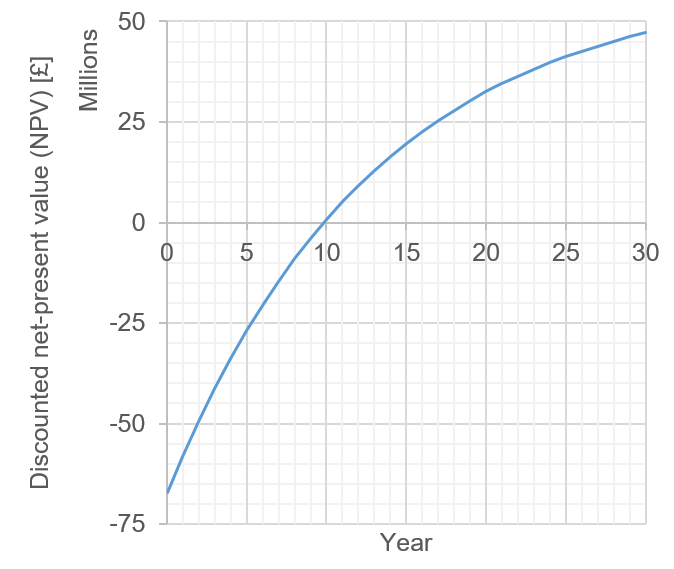
\includegraphics[width=0.5\linewidth]{NPV.png}
%    \caption{Discounted net-present value of the median baseline case operating with a strike price of 100 £/MWh}
%    \label{fig:NPV}
%\end{figure}

%The sensitivity of the adopted strike price to the payback time is presented in Figure \ref{fig:Paybacktime}.

%\begin{figure}
%    \centering
%    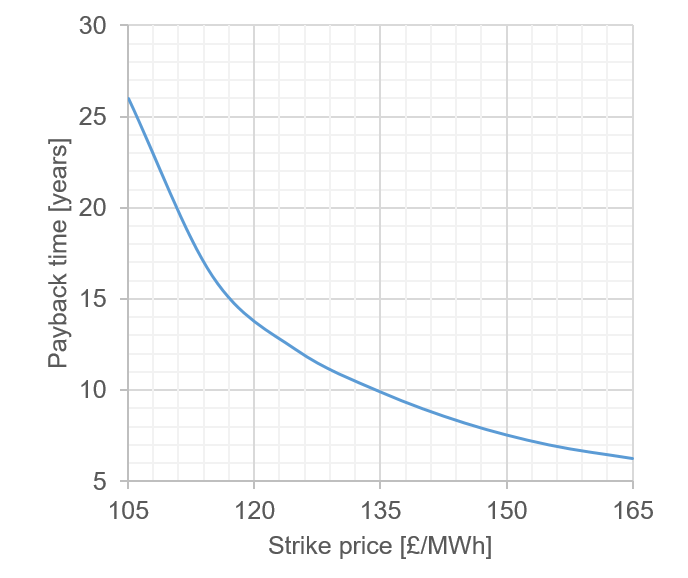
\includegraphics[width=0.5\linewidth]{Paybacktime.png}
%    \caption{Discounted payback time for the median baseline case operating with various strike prices}
%    \label{fig:Paybacktime}
%\end{figure}

\subsubsection{Income Cap \& Floor Model} 
An alternative model might be the so-called Income Cap and/or Floor Model which seeks to minimise losses/profits from the plant to guarantee it is viable whilst protecting consumers. 

Arbitrage trading in the form required for long-duration energy storage would certainly not be expected to be profitable in the current market. However, as presented in Figure \ref{fig:LCOS} this is largely associated with the contribution of capital cost of to the levelised cost of energy storage. 

An operational model might be for the network owner to consider the storage asset to be part of its own wider infrastructure. If for example ownership of the storage assets themselves was held by the network (or government) and operational costs (maintenance, gas, electricity \textit{etc.} were covered by plant revenue then the main challenges of financing and initial equipment purchase would be overcome. Additionally, the operator would be insured against low capital utilisation by the network and could focus on supporting that network for its revenue. 







%to utilise wholesale electricity prices for buying and selling and to incentivise supporting the network directly through arbitrage trading. This market is uncertain, especially over a 30 year lifetime and such a model would certainly not be expected to be profitable in the current market. On the other hand, the security and resilience offered by long duration energy storage simply being available if required has significant value to network operators. Hence an agreement for a minimum monthly income would mean that the storage capacity can be maintained and held online. 

%Revenue could for example cover the base plant CAPEX and OPEX costs not including electricity/gas which could be traded on the wholesale market. Over the 30 year lifetime of the plant, the median baseline scenario would cost £123m paid by the network operator/government. Any plant profits could come from supporting the network through arbitrage trading.

\subsubsection{Regulatory Asset Base (RAB)} 
In this example, a contract is agreed with the Government for a Company to own and operate the plant. The Company pre-agrees a secured but regulated return. This option provided a secure rate of return and thus reduces the risk to an investment. The LCOS analysis presented above has assumed a fixed return of 8\% across the project for investors.

The sensitivity of the investor's return rate on the LCOS is Figure \ref{fig:LCOS-Utilisation}. 

\subsubsection{Capacity Market (CM)} 
The plant operator bids for a contract to offer an agreed energy storage capacity one to four years ahead of delivery. A fixed monthly payment is agreed (per unit of power) with the operator over a fixed time period with contracts up to two years. This insures some revenue to investors but durations are too short to underpin a 30 year investment. However in principle they do offer an potential framework for a revenue model for a P-CAES plant. 

The Short-Term Operating Reserve (STOR) pays energy providers to be available (availability period in £/MW/h) and in their use (utilisation period in £/MWh). These numbers vary depending on market conditions but are typically less than 10 £/MW/h and more than 100 £/MWh for the availability and utilisation payments respectively. Typical figures for the availability payment are 7.34 £/MW/h \cite{zhong2009assessment} and for utilisation payments are averaging 400 £/MWh since November 2017 \cite{nedd2020operating} or were 288 £/MWh \cite{zhong2009assessment} in January 2009 . 

The above figures are likely to change significantly as we move forward as more energy storage solutions will be made available to electrical networks particularly for the short duration energy storage market. However a discounted payback time evaluation of the median baseline case is presented in Figure \ref{fig:NPVCM}. 

The analysis has been performed assuming a cost of finance of 8\%, an availability payment of 5 £/MW/h and utilisation payment of 100 £/MWh for the electricity sold to the network. Based on a a 15\% utilisation rate, this would yield a fifteen year payback time.

\begin{figure}
    \centering
    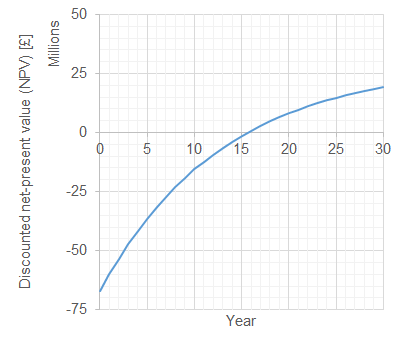
\includegraphics[width=0.5\linewidth]{P-CAES-CapacityMarket-NPV.png}
    \caption{Discounted net-present value of the median baseline case operating with a utilisation payment of 100 £/MWh.}
    \label{fig:NPVCM}
\end{figure}

The utilisation payment obtained here will largely be market driven and thus is uncertain. Hence the sensitivity to payback times is presented in Figure \ref{fig:PaybacktimeCM}. As presented, utilisation payments in excess of 175 £/MWh would yield a payback time of less than 5 years. 

\begin{figure}
    \centering
    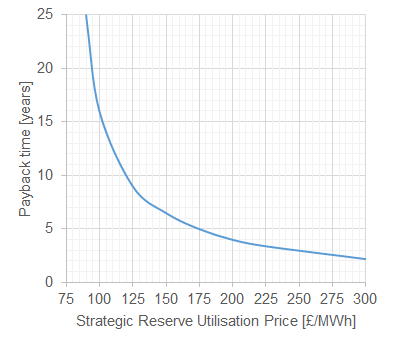
\includegraphics[width=0.5\linewidth]{P-CAES-CapacityMarket-Payback.png}
    \caption{Discounted payback time for the median baseline case operating with various utilisation payment prices.}
    \label{fig:PaybacktimeCM}
\end{figure}

\section{Comparing long-duration energy storage systems}
There a suite of technologies which could be deployed to deliver long-duration electrical energy storage (LDES) in the 5 hours and upwards range. The most promising options are set out by Hunter \textit{et al.} \cite{HUNTER20212077} and an extended list is outlined in Table \ref{tab:FlexPowerSys}. 

\begin{table}[h]
\centering
\begin{tabular}{l p{7.5cm}}
\toprule
\textbf{Acronym} & \textbf{Technology description} \\
\midrule
PHS	& pumped hydropower storage\\
D-CAES | Salt &	diabatic compressed air energy storage in a salt cavern \\
A-CAES | Salt &	adiabatic compressed air energy storage in a salt cavern \\
P-TES &	pumped thermal energy storage\\
VRB	& vanadium redox flow batteries\\
LI-Ion & lithium-ion batteries\\
NG-CT &	natural gas combustion turbine\\
NG-CC &	natural gas combined cycle\\
NG-CC | CCS	& natural gas combined cycle with 90\% carbon capture and sequestration \\
Eth-CC &	ethanol-fuelled combined cycle \\
H2-CC | Salt &	PEM electrolysis, combined cycle, and storage in a salt cavern \\
Stat-PEM | Salt	 & PEM electrolysis,  PEM fuel cell, and storage in a salt cavern \\
HDV-PEM | Salt & PEM electrolysis, heavy-duty vehicle fuel cells, storage in a salt cavern \\
HDV-PEM | Pipes	& PEM electrolysis,  heavy-duty vehicle fuel cells, storage in underground pipes \\
\bottomrule
\end{tabular}
\caption{Flexible power generation systems and LDES systems selected for evaluation}
\label{tab:FlexPowerSys} % Unique label used for referencing the table in-text
% %\addcontentsline{toc}{table}{Table \ref{tab:example}} % Uncomment to add the table to the table of contents
\end{table}

In general terms and as presented in Figure \ref{fig:energystorage}, regardless of whether they store electrochemical, thermal, or mechanical energy or use a chemical fuel, an energy storage technology uses electrical energy as an input and for an output, often requiring a transformation into another form of potential energy for effective storage before recovery back to electricity. Each stage carries its own losses, lifetimes and costs which are detailed in the figure. Additionally, there are challenges associated with system response times, safety \textit{etc.} as well as environmental and social impacts. As systems scale from the kWh to MWh to GWh scales, the significance of some of these parameters can scale disproportionately meaning an evaluation which considers all these factors at the design scale is key to conducting any kind of comparison. 

\begin{figure}
    \centering
    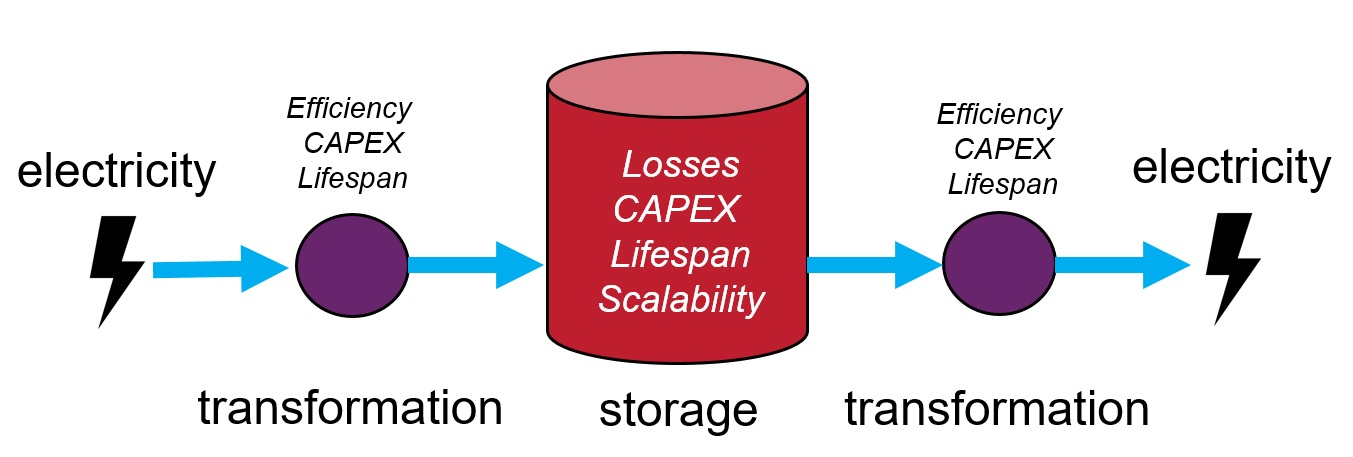
\includegraphics[width=0.8\linewidth]{EnergyStorageSystem.jpg}
    \caption{Block diagram of a generic energy storage system}
    \label{fig:energystorage}
\end{figure}

With so many technologies and each with their own advantages and disadvantages, comparisons require the consideration of multiple and often conflicting parameters \cite{Julch2016}, \cite{HUNTER20212077}. For simplicity whilst providing a wide scope for comparison the following analysis builds upon more comprehensive evaluations of electrical energy storage.

\subsection{Energy storage system size evaluation}

Presented in Figure \ref{fig:energystoragescale} is an evaluation carried out by the World Energy Council \cite{WorldEnergyCouncil2016} of typical energy storage capacities and discharge times at maximum rated power for a suite of energy storage technologies. The outcome reflects the general consensus that capacitors, flywheels and electrochemical batteries (Li-Ion) can deliver smaller scale and rapid response energy storage services to a network. 

However, as systems scale-up beyond 1.0 MWh and to longer storage durations, the relative value of higher round trip efficiencies typically becomes less significant and is outweighed by the need to reduce the engineering complexity, manufacturing intensity and corresponding cost of the storage mediums themselves.  Furthermore, those solutions which can decouple the power capacity from the energy storage capacities are more viable as they can be tailor made to meet the end-user's power demand and duration of storage requirements. 

Most notably, power-to-gas (P2G) technologies (presented here as hydrogen and synthetic natural gas) are generally considered appropriate solutions for large scale and longer duration energy storage. These solutions can be scaled to produce gases which can be stored for extended periods hidden in salt caverns and other geological structures. The same is also true for pumped hydro power albeit with a proportional and usually undesirable re-purposing of the land surface environment in unique geological topographies.

Compressed air energy storage (CAES) systems also support the decoupling of the power and energy components enabling longer storage durations. Typically, the maximum size is limited by the availability and scale of local geographical structures which are usually salt caverns. This capacity can further be increased by operating those systems at higher pressures if possible without affecting their integrity. Nevertheless at smaller scales, storage in pressure vessels is possible. 

The evaluation by the World Energy Council \cite{WorldEnergyCouncil2016} has been extended to include the outcomes of the evaluation presented in Section \ref{sec:EconomicEvalution} on P-CAES. Typically the pipelines presented in Figures \ref{fig:power} and \ref{fig:capacity} would provide the range presented in purple in Figure \ref{fig:energystoragescale}. Compared to conventional CAES in salt caverns, this would place the technology in the 1.0 GWh range with storage durations of between an hour and a month depending on the length of the pipeline and the size of the powerplant. Compared to conventional CAES, which is technically unconstrained by its charging/discharging power as more compressors/turbines can be utilised, a P-CAES system has a maximum pipe flowrate and thus charging/discharge rate. 

\begin{figure}
    \centering
    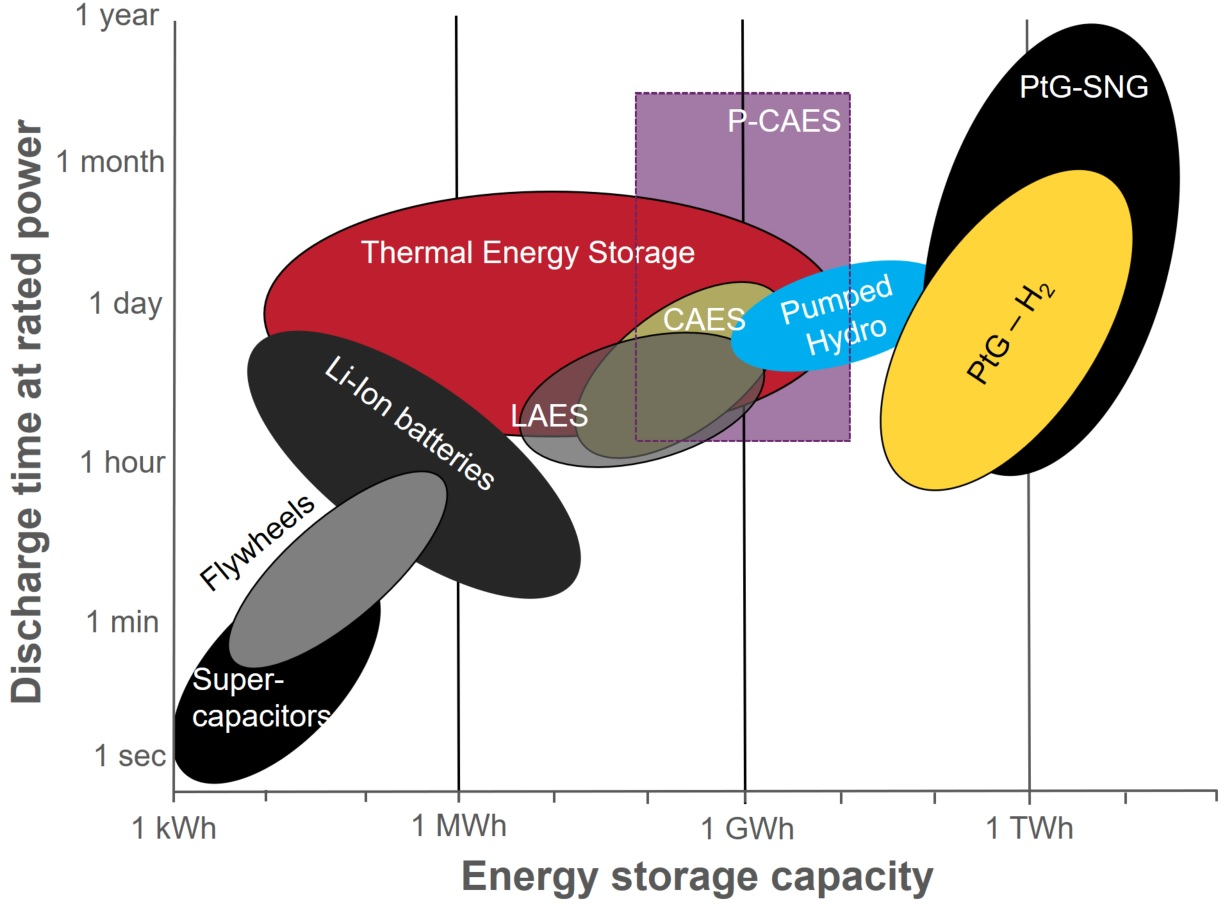
\includegraphics[width=0.8\linewidth]{SystemScale.jpg}
    \caption{Comparison of major energy storage technologies and their Levelised Cost of Storage \cite{WorldEnergyCouncil2016} \cite{Smallbone2017}. 
    \textit{PtG: Power to Gas. SNG: Synthetic Natural Gas. H2: Hydrogen. P-CAES: Pipeline Compressed Air Energy Storage. CAES: Conventional Compressed Air Energy Storage. LAES: Liquid Air Energy Storage.}}
    \label{fig:energystoragescale}
\end{figure}

\subsection{Levelised cost of storage (LCOS) evaluation}

To compare across the various electrical energy storage technology options, a levelised cost of storage (LCOS) evaluation has been performed based upon the assumptions and methodologies set out by Hunter \textit{et al.} \cite{HUNTER20212077}. This recently published study from 2021 developed a database comprised of state-of-the-art data and team of expertise from US Department of Energy and the US National Laboratories to establish a consensus of the most accurate dataset and collective understanding of the challenges of retaining flexibility in a future renewable-rich electricity grid. 

The work explored the technologies listed in Table \ref{tab:FlexPowerSys} based on current costs and performance as well as those expected in the future. Additionally, these researchers have provided open access to their models and data enabling others to perform LCOS and sensitivity evaluations to compare multiple energy storage technologies across a consistent database and well defined methodology.

The published database includes primary inputs to the model including system power output capacity, capital costs, operating and maintenance (O \& M) costs (such as insurance and property taxes), system and component performance and durability, charging electricity and/or fuel costs, storage duration, and capacity factors. 

\subsubsection{Assumptions} 

Using this model and the same database, the modelling analysis carried out and published by Hunter \textit{et al.} \cite{HUNTER20212077} has been repeated and extended to also include a P-CAES system. 

\underline{The future energy system}: The original work included a number of scenarios which are detailed in their publication, however for simplicity and to illustrate the potential of the proposed P-CAES technology, the most detailed scenario explored in this work is adopted. Long-duration energy storage is required to retain resilience and flexibility in a electricity market with a high proportion of renewable energy. This scenario is set out in in Table \ref{tab:CounterfactualScenerio}. 

\begin{table}[h]
\centering
\begin{tabular}{l c}
\toprule
\textbf{Parameter [Units]} & \textbf{Value}\\
\midrule
Power Capacity [MW]	& 100\\
Electricity Market [-]	& Western United States\\
Renewable electricity penetration [\%]	& 85\\
Other electricity sources [-] & Natural gas spinning equipment, coal, and nuclear.\\
Charging electricity price [\$/MWh]	& 20\\
Charging capacity factor [\%]	& 27\\
Discharging capacity factor [\%]	& 15\\
\bottomrule
\end{tabular}
\caption{Summary of the parameters used in the LCOS evaluation across storage technologies.}
\label{tab:CounterfactualScenerio} % Unique label used for referencing the table in-text
% %\addcontentsline{toc}{table}{Table \ref{tab:example}} % Uncomment to add the table to the table of contents
\end{table}

Electric grids with renewable sources market penetration levels exceeding 80\% will likely require long duration energy storage or flexible, low-emission power generation to balance supply and minimize costs while meeting demand. Hence, an 85\% renewable electricity market penetration is considered based around the energy market of the Western United States. This corresponds to 19\% hydropower, 28\% solar power, 33\% wind power, 4\% geothermal \textit{etc.} \cite{Zhangetal}. The remaining (circa. 15\%) was considered to be comprised of natural gas spinning equipment, coal, and nuclear. 

It is not expected that the energy storage system will be used continually, it generally will support the wider energy system by operating during those times of mismatched supply and demand mainly driven by external weather-driven and electrical demand factors. Determining the frequency and the nature of the utilisation of the storage system is therefore quite complex and thus it is challenging to estimate based on a hypothetical future energy system. For example, in the real-world, the corresponding costs will be dynamic and market driven. Additionally many key and competing future energy technologies are uncertain in terms of policy incentives, rates of deployment, performance, cost parameters \textit{etc.} 

Nevertheless to address this challenge, Hunter \textit{et al.} \cite{HUNTER20212077} utilises the same optimal dispatching sub-model developed by Zhang \textit{et al.} \cite{Zhangetal}. Presented in Figure \ref{fig:zhangetal} is a visual summary of the net-change in the state-of-charge for an energy storage system with a RTE=40\%. The figure shows that over any one given week, in the spring months the storage system would generally be charged toward full and conversely discharged over the autumn toward empty. However over a typical day and taking advantage of daily demand fluctuations, a storage system would take advantage of night time charging and return value from daytime discharging. However, more uncertain storage system utilisation is observed in the high summer and winter months.

\begin{figure}
    \centering
    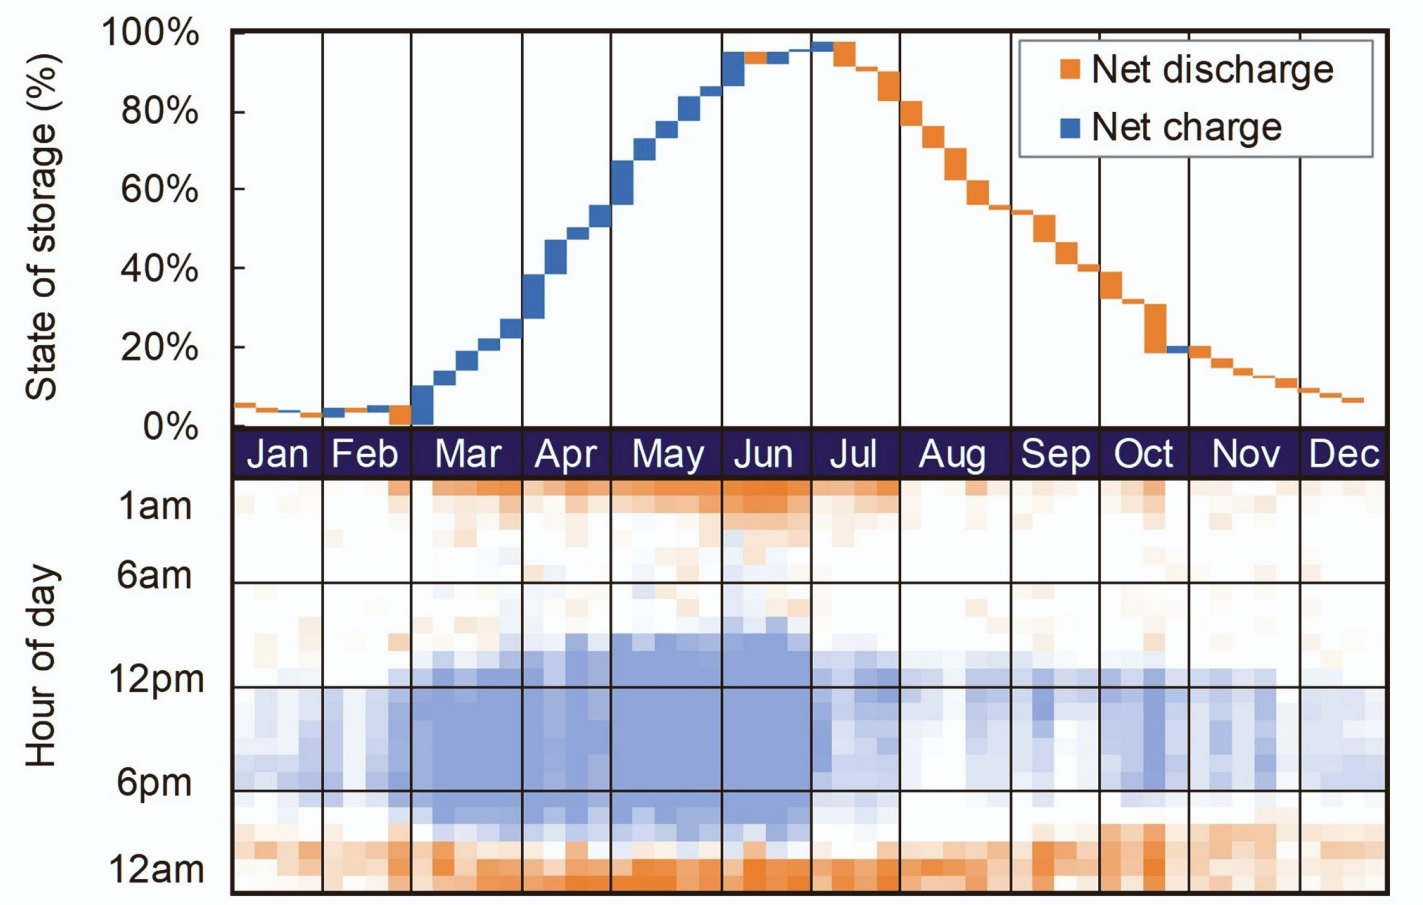
\includegraphics[width=0.8\linewidth]{Zhangetal.jpg}
    \caption{ Daily and weekly storage cycling for a long duration energy storage system in the Western United States with 40\% round-trip efficiency according to Zhang \textit{et al.} \cite{Zhangetal}.}
    \label{fig:zhangetal}
\end{figure}

The adopted optimal dispatching model accounts for (RT) efficiencies and likely charging, storage and discharge profiles. The analysis brings forward correlations between storage system RTE and optimal corresponding charging and discharging capacity factors. The output are estimates for charging and discharge capacity factors which have been defined on a storage technology specific basis. 

Two forms of CAES are also included in the analysis by Hunter \textit{et al.} \cite{HUNTER20212077} and Zhang \textit{et al.} \cite{Zhangetal} and the numbers used for D-CAES have been adopted for the current analysis due to the very similar technical and operational performance expected for P-CAES. The outcome is that the required charging and discharge capacity factors have been estimated as 27\% and 15\% respectively. 

\underline{System performance and economic parameters}: The key performance and economic parameters used in analysis by Hunter \textit{et al.} \cite{HUNTER20212077} are presented in Table \ref{tab:CounterfactualCosts}. Figures are based around a baseline of US dollars in 2018. Fixed costs do not include a property tax and insurance of 1.5\% of CAPEX.

\begin{table}[h]
\centering
\begin{tabular}{l c}
\toprule
\textbf{Parameter [Units]} & \textbf{Value}\\
\midrule
CAPEX - Charging system component [\$/kW]	& 507 \\
CAPEX - Discharging system component [\$/kW] & 759 \\
\midrule
OPEX - Fixed charging system component [\$/kW-yr] & 13.5 \\
OPEX - Fixed discharging system component [\$/kW-yr] & 13.5 \\
OPEX - Variable discharging system component [\$/MW] & 3.3 \\
\midrule
Round trip efficiency [\%]	& 55\\
System lifetime [years]	& 30\\
\bottomrule
\end{tabular}
\caption{Key CAES parameters \cite{HUNTER20212077} used in the counterfactual analysis.}

\label{tab:CounterfactualCosts} % Unique label used for referencing the table in-text
% %\addcontentsline{toc}{table}{Table \ref{tab:example}} % Uncomment to add the table to the table of contents
\end{table}

In general, the analysis \cite{HUNTER20212077} presents a generic set of state-of-the-art parameters for estimating the likely performance and costs of a CAES system for installation in the US. These figures differ slightly from those presented and used in Section \ref{sec:EconomicEvalution} however differences are not significant enough to justify re-running simulations for the D-CAES and A-CAES energy storage systems. Indeed it would have been possible to utilise the data developed in the analysis presented in earlier Sections to reflect a more detailed evaluation of CAES in its different permutations. However when put in context with other uncertainties associated with capacity factors, cost performance \textit{etc.}, it was not deemed as important as retaining a common, previously peer reviewed methodology and data set for the comparisons. Instead for the evaluation of the P-CAES system the baseline D-CAES system parameters were adopted with the original costs of storage associated with geological salt storage modified to those presented in Section \ref{sec:EconomicEvalution}.

\subsubsection{Model results and analysis}  

The analysis indicates that the opportunities to charge the system are often more frequent to those for discharging. It suggests that a more optimal energy storage system design would mean that the total power of the turbine powertrain would greater the compressor power \textit{i.e.} that charging would take longer than discharging. The parameters of the optimal storage system for the proposed energy system are presented in Table \ref{tab:CounterfactualP_CAES}.

\begin{table}[h]
\centering
\begin{tabular}{l c}
\toprule
\textbf{Parameter [Units]} & \textbf{Value}\\
\midrule
Charging power capacity [MW] & 55.35 \\
Discharging power capacity [MW]	& 100 \\
Storage durations [hours] & 1 - 168\\
Storage durations [MWh] & 119 - 20080\\
\bottomrule
\end{tabular}
\caption{Summary of the optimal sizing of a 100MW P-CAES system for the Western United States with an 85\% renewable electricity market.}

\label{tab:CounterfactualP_CAES} % Unique label used for referencing the table in-text
% %\addcontentsline{toc}{table}{Table \ref{tab:example}} % Uncomment to add the table to the table of contents
\end{table}

Similarly corresponding data to support and equivalent analysis of all the options presented in Table \ref{tab:FlexPowerSys} has been carried out by Hunter \textit{et al.} \cite{HUNTER20212077}. The result of all these analysis are presented in Figure \ref{fig:counterfactual} in terms of the levelised cost of storage. The diagram summarises the unit cost of storage for each technology at a fixed 100MW power output capacity when increasing storage durations from an hour to 168 hours (seven days).  

\begin{figure}
    \centering
    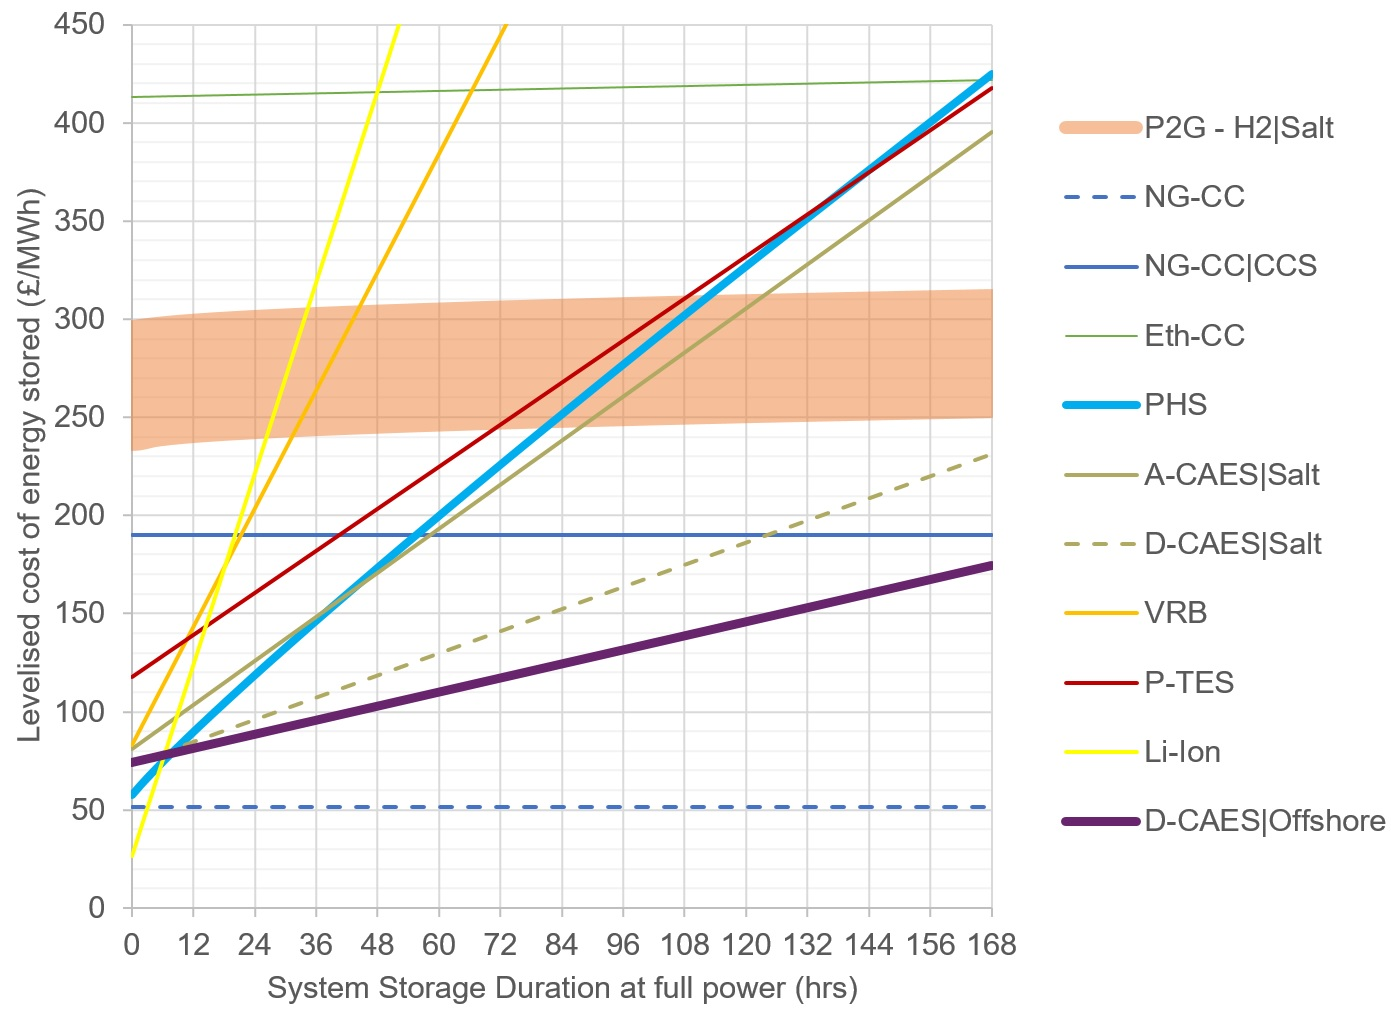
\includegraphics[width=0.8\linewidth]{Counterfactual.jpg}
    \caption{Levelised cost of storage (LCOS) comparison for different storage durations between different energy storage technologies}
    \label{fig:counterfactual}
\end{figure}

To simplify the diagram, the energy storage technology permutations which included storing hydrogen in salt caverns have been collated into an orange band. The diagram shows a number of clear trends across the types of storage medium, conversion technologies \textit{etc.} and how they scale with storage duration.

For shorter storage durations (and considering the block diagram of Figure \ref{fig:energystorage}), overall storage costs are generally dominated by the capital cost of the technology used for transformation to storage and from storage to electricity. At sub- 8 hours of storage, lower costs for PHS and Li-Ion batteries are most favourable but as storage durations increase, the relative cost of the storage medium becomes more dominate in terms of LCOS. The gradients of the lines are proportional to the cost of storage media and as presented, the relative costs of Li-Ion and VRB battery technologies quickly become economically unfavourable for longer storage durations.

The relative cost of the storage medium is much less significant for solutions involving natural gas, hydrogen and ethanol and gradients are lower. Nevertheless, they all carry high transformation system capital costs which mean that they only become economically favourable as storage durations lengthen.

The permutations of CAES offer a balance of both relatively low CAPEX for the transformation system and for the storage media. In all cases of D-CAES, A-CAES and P-CAES, economically favourable opportunities in the 8-168hrs storage regimes are apparent. Principally, due to a lower cost of storage medium, the P-CAES offers the most potential to deliver low-cost energy storage at scale.

\section{Conclusions}
In this analysis, a techno-economic assessment for energy storage from re-purposed fossil-fuel era infrastructure has been completed. This was completed by means of using offshore UKCS oil and gas pipelines as the pressure vessel in conventional D-CAES plant. A technical feasibility evaluation has been conducted. 

A thermodynamic model based on energy flows was presented for assessing the storage capacity and required turbomachinery. This gave an estimate of the scale of energy storage available at each of the major pipeline landings. 

The Levelised Cost of Storage (LCOS) was then analysed and found to be competitive with other energy storage methods and conventional CAES systems. A range of specific recommissioning, system CAPEX and OPEX costs were presented, representing the estimated level of uncertainty observed. A detailed benchmarking evaluation was carried out comparing the various technical options, it proved that that long duration energy storage system costs are highly sensitive to utilisation frequency and the relative costs of the storage medium. 

%\appendix

%% If you have bibdatabase file and want bibtex to generate the
%% bibitems, please use
%%
 \bibliographystyle{elsarticle-num} 
 \bibliography{cas-refs}

%% else use the following coding to input the bibitems directly in the
%% TeX file.

% \begin{thebibliography}{00}

% %% \bibitem{label}
% %% Text of bibliographic item

% \bibitem{}

% \end{thebibliography}
\end{document}
\endinput
%%
%% End of file `elsarticle-template-num.tex'.
